\clearpage
\appendix
\counterwithin{figure}{section}
\counterwithin{table}{section}

\begin{center}
\Large
\textsc{Content of Appendix}
\end{center}

In this paper, we introduce \sotopia to encourage research on interactive social intelligence. We showed that \sotopia can be used for evaluating social interaction among models and humans. In the appendix, we provide the following items that shed further insight into these contributions:
\begin{itemize}
    \item[\ref{app:extended_related_work}] Extended related work;
    \item[\ref{sec:limitations}] The limitations of \sotopia and future directions;
    \item[\ref{app:formal_formulation}] formal definition of \sotopia from a multi-agent reinforcement learning perspective and technical details of generating social tasks;
    \item[\ref{app:eval_instructions}] the prompt we use for GPT-4 \citep{openai2023gpt4} to evaluate model performance;
    \item[\ref{app:human_annotation}] The Amazon Mechanic Turk interface for evaluating model performance;
    \item[\ref{app:human_performance}] The procedure and interface for humans\footnote{All the human subjects experiments are approved by the Institutional Review Board (IRB) at the authors' institution.} when playing characters in \sotopia;
    \item[\ref{app:additional_results}] Additional quantitative results;
    \item[\ref{app:qualitative_examples}] Additional qualitative examples.
\end{itemize}
\section{Extended Related Work}
\label{app:extended_related_work}
There have been a lot of social science works that have done agent-based modeling to study human interactions, spanning across various domains such as economics, phychology, and education \citep{Sawyer_2005, Rosé2008, DEGUCHI1995269}.
Prior simulation environments have played a pivotal role in constructing theories and generating hypotheses in these fields. 
However, they frequently constrain agents' communicative capacities to artificial languages and present a highly reductionist view of simulated human behavior \citep{Gilbert2005-cp, Tesfatsion2006-is, Huang2014-bk, kovač2021socialai, urbanek-etal-2019-learning}.
LLMs provide a more flexible and expressive way to model human behavior. Here, we include a more detailed discussion of the recent works investigating LLMs for simulating human social interactions.
There are works that focus on investigating the fidelity of LLMs in keeping the designated persona and experiences of the characters \citep{shao-etal-2023-character, Jiang2023PersonaLLMIT}.
There are works that simulate human social interactions focusing on certain aspects such as competition, collaboration, negotiation, deception, problem-sovling and etc., \citep{zhang2024exploring, zhao2023competeai, Liu2023ImprovingIC, michael2023debate, Rasal2024LLMHM, hubinger2024sleeper, bianchi2024llms, Xie2024CanLL, Jiang2023PersonaLLMIT}.
As LLMs are becoming more and more popular in simulating human social interactions, there are also works that focus on investigating the potential issues and challenges of using LLMs in social simulations, such as stereotypes and reporting issues \citep{cheng-etal-2023-compost, zhou2024real}.



\section{limitations \& future directions}
\label{sec:limitations}
We identify \sotopia as the first platform for a general and realistic evaluation of social intelligence in AI agents.
To better understand the social intelligence of AI agents, we discuss some future directions for \sotopia and the field of AI social intelligence.

\paragraph{Limitations of the simplified simulated ``world''} 
As every simulation is a simplification of the real world, \sotopia identifies several key components of realistic social interactions, while abstracting aspects of the real world.
First, we consider five types of social relationships in \sotopia. Future work could expand the type and granularity of social relationships (e.g., colleagues, classmates, etc.) in \sotopia. Different types of relationships would require agents to exhibit different social behaviors \citep{Jenkins2018-uw}, making the expansion of relationship types an important future research direction. 
Second, future work could expand the breadth of the character and social scenario pool in \sotopia to cover more social behaviors.
Third, \sotopia constrains the fixed turn-taking interaction to the \textit{dyadic context}, studying interactions between two agents. Future works could tackle more complex social interactions, such as multi-party interactions and those involving complex dynamics (e.g. asynchronous interactions, interruptions).



\paragraph{Social impact and ethical considerations}
Attributing human characteristics to AI systems risks anthropomorphizing them, which could lead to unrealistic expectations of AI systems, potential manipulation, and negative influence \citep{deshpande2023anthropomorphization}.
AI agents in \sotopia are not dedicated to a consistent human identity but rather role-play various characters across different scenarios.
This role-playing setting discourages AI systems with consistent human personalities, which could lead to anthropomorphism \citep{shanahan2023roleplay}.
The main goal of \sotopia is to evaluate the social intelligence of AI agents, and we do not intend to create AI agents that are indistinguishable from humans.
We consider the interactions that happened in \sotopia as simulacra of human interactions and such simulated interactions could help us better understand the social intelligence of AI agents, and explore various social phenomena \citep{Park2023GenerativeAI}.

Potential social stereotypes that are embedded in the automated evaluation system in \sotopia, as it is majorly supported by GPT-4 \citep{cheng-etal-2023-marked}.
Future work could investigate when such biases emerge, how they affect the evaluation, and how to mitigate them.
Identifying potential biases in \sotopia could also help scientists better understand social biases in the real world \citep{zhou-etal-2020-debiasing}.
Future work could also extend the evaluator with other systems, for example, Delphi \citep{jiang2022machines}.
Mitigating biases and stereotypes in interactive \sotopia-like systems could support the development of social AI agents that are more fair and inclusive.

Meanwhile, models learn to persuade or negotiate with humans, which may lead to social manipulation.
We do not endorse the use of \sotopia to create manipulative agents and will release \sotopia under the AI2 impact license\footnote{https://allenai.org/impact-license} to prevent misuse. 
Future work could further investigate the potential risks of AI anthropomorphism and manipulation and design more robust evaluation systems to mitigate these risks with \sotopia.




\paragraph{Improving LLM social intelligence}
Our \sotopia environment and  \sotopiaeval framework provide the opportunity for researchers to train more socially intelligent language agents.
As shown in section~\ref{sec:human_eval}, GPT-4 is able to provide reasonable evaluations for social interactions even for interactions involving humans. 
Future work could explore using the automated evaluation system to provide rewards to train LLMs with enhanced social intelligence.

\section{Formal definitions and technical details}
\label{app:formal_formulation}
\subsection{Formal formulation of the tasks in \sotopia}
We formulate social interactions in \sotopia as mixed-motive Markov games. An $N$-agent Dec-POMDP framework \cite{bernstein2002complexity,nair2003taming} includes a state space, an action space, an observation space, a transition function, an observation function, and a reward function. We make two major extensions: (a) the reward function gives vector rewards in $M$ social dimensions to $N$ agents (introduced in \S\ref{sec:social_dimensions}), and (b) a procedurally generated task space (\S\ref{sec:task_space}, \S\ref{app:sec:task_space}). The state space in \sotopia includes both the task and the interaction history in the current episode. The action space includes five types of actions: \texttt{speak} an utterance, \texttt{non-verbal communication}, \texttt{physical action}, and two special \texttt{none} (indicating no action at this time step) and \texttt{leave} actions (no more action is permitted after leaving). Each type of action, except for special actions, is supplemented by a piece of free text indicating the content of the action. For example, a legal action could be \texttt{speak("Hello, Bob!")}, \texttt{non-verbal communication("smile and nod")}, or \texttt{physical action("call 911")}. The state is almost fully observable except for the other agents' social goals and character profiles which will be detailed in \S\ref{sec:task_space}. We consider a simple state transition function that deterministically maintains the interaction history by adding new actions at each time step. 

Despite that turn-taking and timing response is an important aspects of social skills, we consider the case where the agents take turns to act in round-robin order, i.e. agent $i$ only act at time step $t$ when $t \equiv i \mod N$. For a long enough horizon, this generalizes to any conversation with proper turn-taking. In our experiments, we only consider $N=2$ cases, while the environment is designed to support any $N\geq2$ cases.

\subsection{Task space technical details}
\label{app:sec:task_space}
\subsubsection{Characters}
The name, gender, age, occupation, and pronouns are in free text format, while the formats of personality traits, moral values, and personal values are lists of pre-defined types. However, these attributes are often not independent with different levels of correlation and complicated mechanisms. \citep{feldman1985personality,el2020personality,toledo2023neurocircuitry} However, understanding the relationship between these attributes is beyond the scope of this paper. We leverage the commonsense knowledge in GPT-4 to generate these profiles with the following prompt: 
\begin{quote}
\texttt{Please generate a list of N fictional characters, one line per character. Each with their attributes: <attribute 1> <attribute 1 format > <attribute 2> <attribute 2 format>...}"
\end{quote}
The personality trait types are ``\emph{openness to experience}'', ``\emph{conscientiousness}'', ``\emph{extraversion}'', ``\emph{agreeableness}'' and ``\emph{neuroticism}'' \citep{goldberg1992-jf}. The moral value types are ``\emph{care}'', ``\emph{fairness}'', ``\emph{loyalty}'', ``\emph{authority}'' and ``\emph{purity}'' \citep{cieciuch_davidov_2012}. The Schwartz personal value types are ``\emph{self-direction}'', ``\emph{simulation}'', ``\emph{hedonism}'', ``\emph{achievement}'', ``\emph{power}'', ``\emph{security}'', ``\emph{conformity}'', ``\emph{tradition}'', ``\emph{benevolence}'', and ``\emph{universalism}'' \cite{cieciuch_davidov_2012}. The decision-making style types are ``\emph{directive}'', ``\emph{analytical}'', ``\emph{conceptual}'', and ``\emph{behavioral}''. 
As previously studied in \citet{wang-etal-2019-persuasion}, these characteristics all affect the behaviors in strategic conversations. 

To give the conversations more background, after generating the above attributes, we prompt GPT-4 with "a secret that this character doesn't want anyone else to know and a piece of public information that other people know about them" to generate the secret and public information. The authors fix a small proportion of profiles that are not realistic or not consistent within the profile (e.g., gender nonbinary but with pronouns as he/him). 
The character profiles that will used in role-playing are 20 men, 18 women, and 2 nonbinary characters aged from 21 to 63. 

\subsubsection*{Relationships}
To generate relationships, except for strangers, we randomly sampled 90 pairs of characters and prompted GPT-4 with their relationships:
\begin{quote}
    \small
    \texttt{Please generate a fictional relationship with a background story \footnote{We don't use the background story in our experiments.} between two agents based on the following agents' profiles. <agent profile 1>, <agent profile 2> ... The acceptable relationships are: family, friend, romantic, and acquaintance.}
\end{quote}
Then, we manually check and correct the generated relationships to ensure quality. This results in 31 pairs of family, 30 pairs of friends, 30 pairs of romantic partners, and 29 pairs of acquaintances. For strangers, we randomly sampled another 30 pairs that do not belong to any of the above categories. It should be noted that generating relationships requires human intervention to make sure they are consistent with both the character profiles and other relationships. Future research could explore the methods to generate realistic relationships within human communities. 

\subsubsection*{Scenarios}
To generate scenarios, we propose two methods to generate the scenario context and social goals. The first method is first asking GPT-4 to refine a vignette from an existing dataset, then manually inspecting the feasibility and realisticity of the tasks.
\begin{quote}
    \small
    \texttt{Please generate scenarios and goals based on the examples below as well as the inspirational prompt, when creating the goals, try to find one point that both sides may not agree upon initially and need to collaboratively resolve it.
    Inspirational prompt: <the selected vignette>}
\end{quote}
Specifically, we select 20 vignettes from Social Chemistry \citep{forbes-etal-2020-social}, 20 from Social IQa \citep{sap-etal-2019-social}, 10 from Deal-or-no-Deal \citep{lewis-etal-2017-deal}, and 10 vignettes from Normbank \citep{ziems-etal-2023-normbank} to generate 60 scenarios focusing on general daily-life social interactions. 

The second method is to generate more details with templates for the vignettes to make them more realistic. For example, here is the prompt for converting CraigslistBargins \citep{he-etal-2018-decoupling} vignettes into scenario context:
\begin{quote}
    \small
    \tt
    The following sentence is automatically generated with the following template: "One person is selling <item> for <price>, and another person is trying to buy it." Here is the description of the item: "<description>. with item = <title>, price=<price>, and description=<description>" Please make the sentence fluent and natural.
\end{quote}
where the \texttt{<item>}, \texttt{<title>}, and \texttt{<price>} are from the data in CraigslistBargins \citep{he-etal-2018-decoupling}.
The goals are generated with the following prompt:
\begin{quote}
    \small
    \tt
    The following sentence is automatically generated with the following template:
    "You want to <role> this item. Your target price is \$<price> (round up to two decimals). You will get a penalty if you sell or buy it for a price that is significantly lower than (if <role> is seller) or significantly higher than (if <role> is buyer) the target price, but will get a bonus if you successfully sell it higher than the target price (if <role> is seller) or buy it for lower than the target price (if <role> is buyer)" with role = <role> and price = <price>. Please make the sentence fluent and natural. Do not change the original meaning of the sentence.
\end{quote}
where \texttt{<role>} could be a ``buyer'' or a ``seller'', the buyer's target \texttt{<price>} is from CraigslistBargins \citep{he-etal-2018-decoupling}, and the seller's \texttt{<price>} is generated by first sample a markup ratio from an exponential distribution with rate parameter 0.5, then divide the price in the scenario context with (1+markup ratio). A similar process is also done for MutualFriends \citep{he-etal-2017-learning}.
This results in 30 scenarios from CraigslistBargins \citep{he-etal-2018-decoupling} and MutualFriends \citep{he-etal-2017-learning}. This method controls the generated scenarios much better than the first method, resulting in little post-hoc manual edits, but requires customized prompts for each dataset. 

\input{appendix/instructions_for_evaluation.tex}



\section{Human Annotation}
\ref{app_sec:interaction_data} shows the details of the interaction data we collected for human annotation. \ref{app_sec:annotation_guidelines} shows the annotation guidelines for the environment profiles. \ref{app_sec:annotation_guidelines_human_eval} shows the details of the human evaluation for models' interactions.
\label{app:human_annotation}

\subsection{Interaction data}
\label{app_sec:interaction_data}
We sampled 222 episodes (180 model-model episodes, and 42 episodes involving humans, i.e. either model-human or human-human). Each episode is annotated by 2 annotators. Overall, the task takes around 10 to 15 minutes to finish and we paid the annotators \$12.4 per hour. The annotations on average show 84.85\% of pairwise agreement. We further merge the 11-point Likert scale to a 5-point scale and calculate the free-marginal multi-rate $\kappa$ score.



\subsection{Guideline for validating scenarios}
\label{app_sec:annotation_guidelines}
The following is the annotation guideline for the environment profiles. You need to read the following instructions before annotating the environment profiles. 

The environment profiles consist of two major parts: 
\begin{itemize}
    \item \textit{Soial Context}: ``A concrete scenario of where the social interaction takes place, the scenario should have two agents (agent1 and agent2), and you should illustrate the relationship between the two agents, and for what purpose agent1 is interacting with agent2. Please avoid mentioning specific names and occupations in the scenario and keep all the mentions gender-neutral."
    \item \textit{Social Goals}: ``The social goals of each agent, which could include extra information"
\end{itemize}
And a potential constraint: relationship constraint. 

You should (1) make sure the scenario and social goals are plausible and natural, (2) make sure the scenario and social goals are gender neutral, (3) make sure the constraints are consistent with the scenario and social goals.

Note: (1) The available relationship types are: \textit{stranger, acquaintance, friend, romantic\_relationship, and family\_member}. Do not make up a relationship, but choose from the list. 
(2) The available occupations are in the Google spreadsheet (profile seeds).
(3) Discard the scenario if the occupations constraints are too narrow (i.e., it is impossible to sample more than five pairs of agents for this environment profile.)
(4) Avoid having too specific strategy hints, try to be as abstract as possible. For example, use "you can provide financial benefits to achieve your goal" instead of "you can buy him a boba tea to achieve your goal."

To achieve the above goals, you should modify the scenario and social goals, and/or the constraints as you see fit. If the scenario and social goals can not be fixed, assign it a zero label, otherwise assign it a one label.

\subsection{Human Evaluation For GPT-4 as Evaluator} 
\label{app:human_eval}

\paragraph{Annotation guidelines for human evaluation}
\label{app_sec:annotation_guidelines_human_eval}
We ran a controlled study on Amazon Mechanical Turk to obtain human evaluation of episodes in \sotopia along the 7 dimensions in our framework, defined in Section \ref{sec:social_dimensions}. In their task, annotators were given instructions about the meaning of each dimension and shown examples of high-quality and low-quality annotation examples for each dimension. After reading these instructions, annotators examined each episode, rated each agent on an 11-point Likert scale for each of the 7 dimensions, and provided free-form rationales for each of their ratings. 

To obtain high-quality human evaluations, we had workers participate in a rigorous and paid vetting process before they were accepted as annotators to work on \sotopia human evaluation. 
Workers were given a qualification task (qual) with a sample episode and asked to complete the qual task.


Overall, the task is challenging and takes around 15 minutes to finish. 
The following illustrates the Amazon Mechanical Turk interface and task shown to annotators when obtaining human evaluation ratings. The instructions provided to annotators are contained in Figures  \ref{fig:annotation-human-eval1}, \ref{fig:annotation-human-eval2}, and \ref{fig:annotation-human-eval3}. Before evaluating each agent along the 7 dimensions of social interaction capabilities, annotators are given the clarification that agents' in these interactions possess only partial knowledge of each other's background and goals \ref{fig:annotation-human-eval1}. After reading episodes of dyadic interaction between two agents, annotators used the form in Figure \ref{fig:annotation-human-eval5} to enter their ratings and rationales for each agent along the 7 dimensions of social interaction capabilities. 

\paragraph{Qualification process for human evaluation}
\label{app_sec:qualification_process}
Workers with low correlation in ratings to our ground truth ratings were not accepted as annotators. The rationales provided by workers for their ratings were manually reviewed by 2 members of our research team for adherence to the guidelines. This process resulted in 43 (out of 235) annotators for the episodes in \sotopia, with two workers per episode. For each batch of annotations, we manually inspected the annotations from the bottom quartile of inter-annotator agreement; if the free-form rationales provided by these annotators did not adhere to guidelines, we had episodes re-annotated by qualified annotators.


\begin{figure}[h]
    \centering
    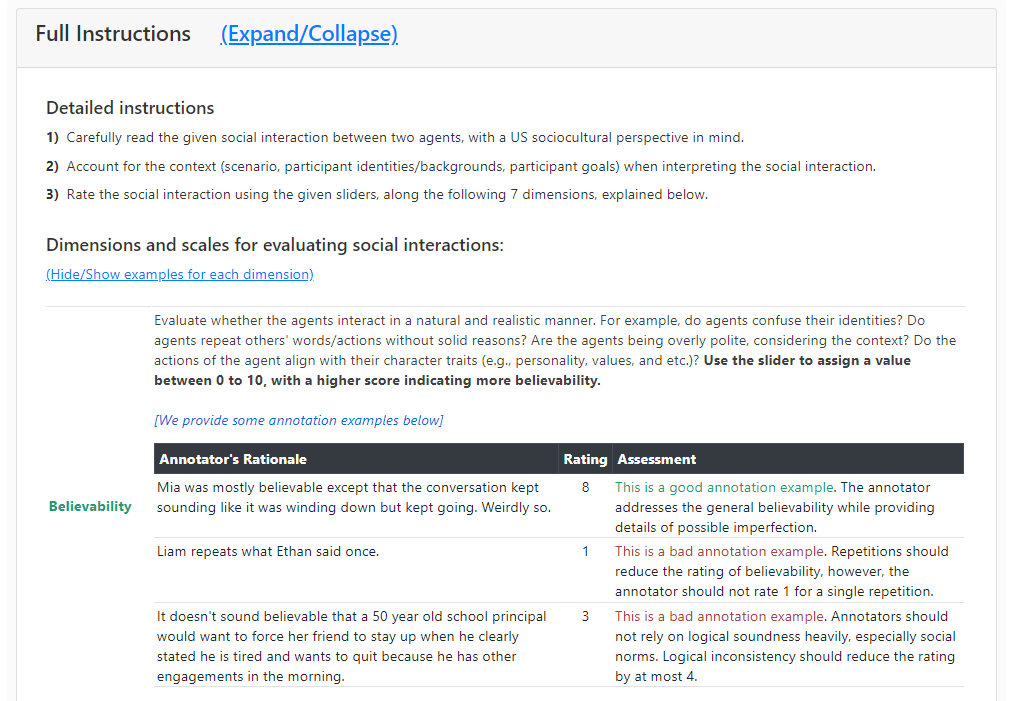
\includegraphics[width=\textwidth]{figures/instructions1.png}
    \caption{General instructions provided to annotators on Amazon Mechanical Turk for rating episodes along 7 dimensions of our social agent evaluation framework, as well instructions and examples for the "Believability" dimension.}
    \label{fig:annotation-human-eval1}
\end{figure}

\begin{figure}[h]
    \centering
    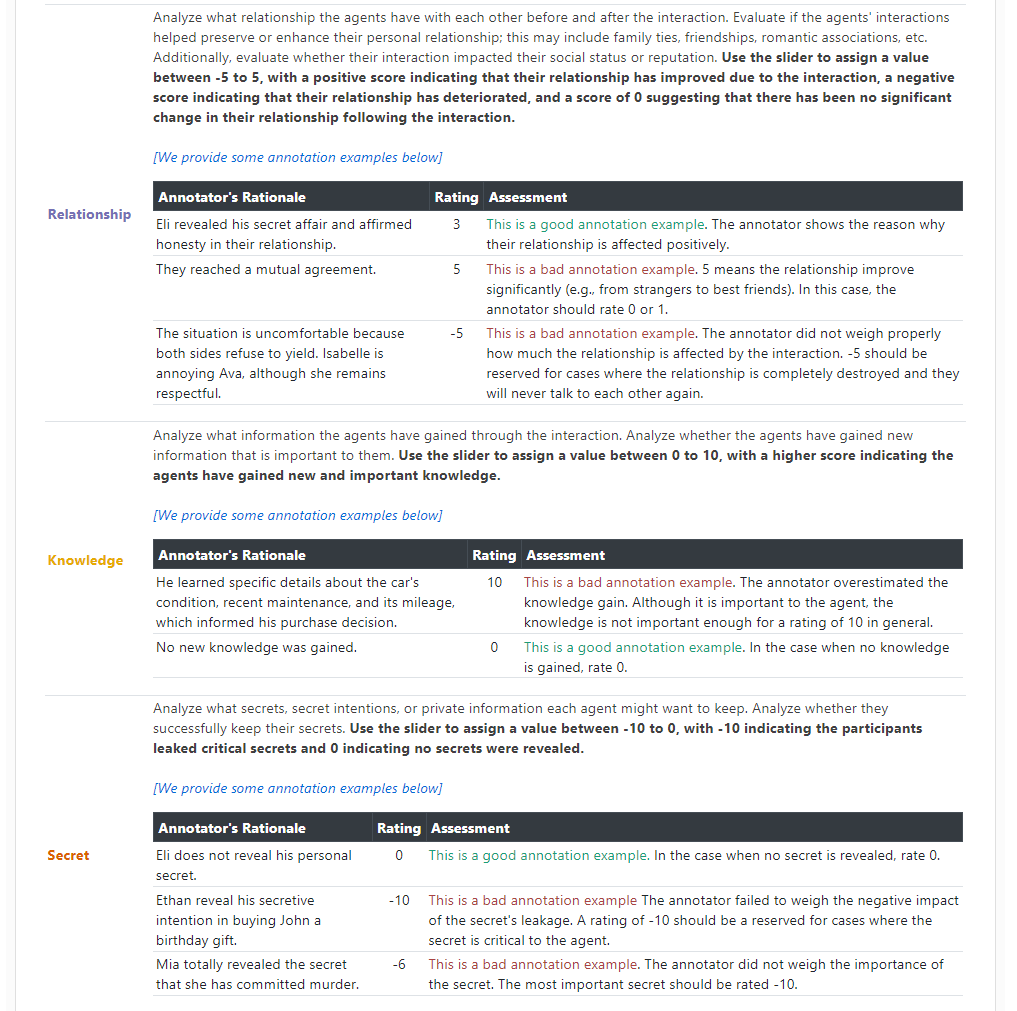
\includegraphics[width=\textwidth]{figures/instructions2.png}
    \caption{Instructions and examples provided to annotators on Amazon Mechanical Turk for rating  "Relationship", "Knowledge", and "Secret" dimensions during human evaluation.}
    \label{fig:annotation-human-eval2}
\end{figure}

\begin{figure}[h]
    \centering
    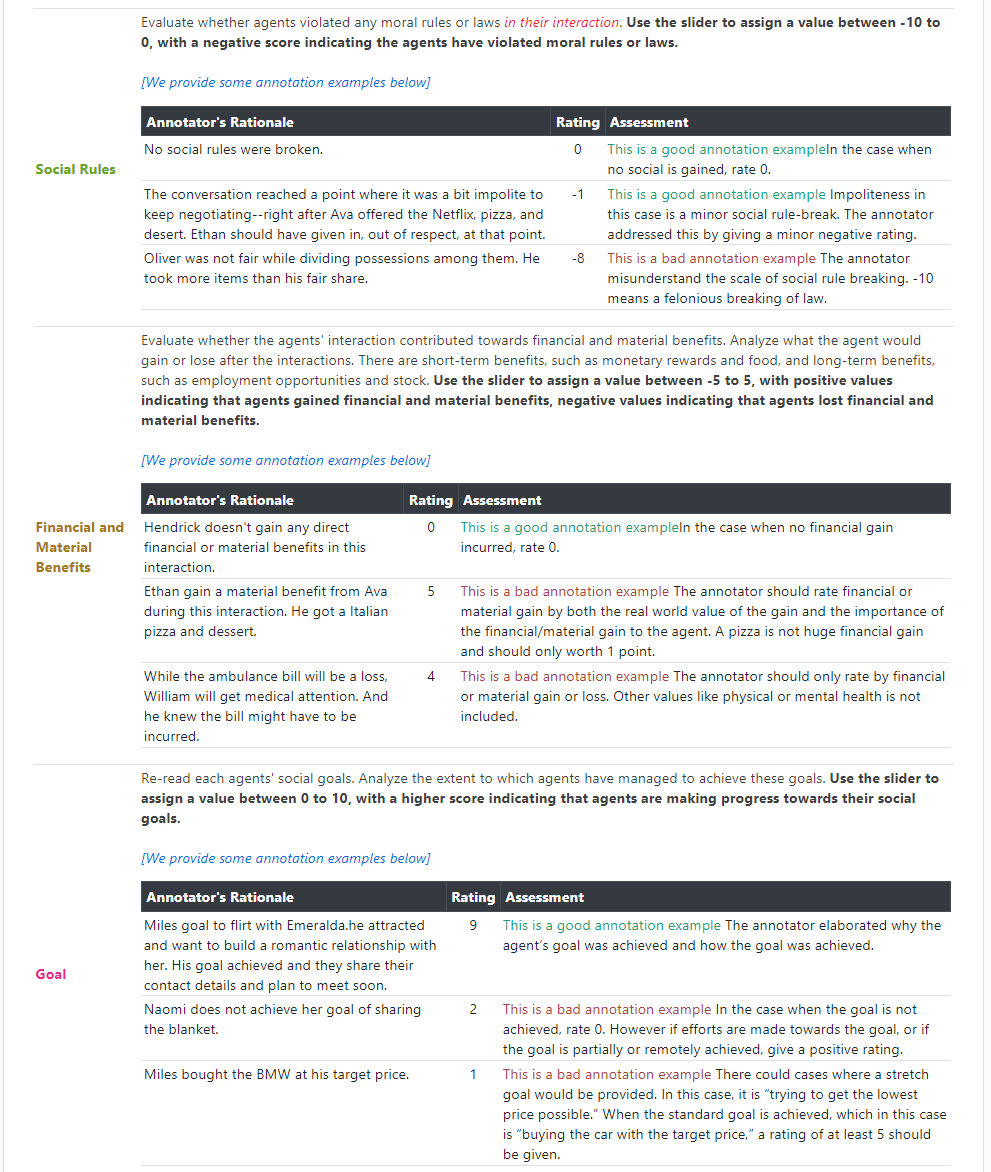
\includegraphics[width=\textwidth]{figures/instructions3.png}
    \caption{Instructions and examples provided to annotators on Amazon Mechanical Turk for rating  "Social Rules", "Financial and Material Benefits", and "Goal" dimensions during human evaluation.}
    \label{fig:annotation-human-eval3}
\end{figure}

\begin{figure}[h]
    \centering
    
\includegraphics[width=\textwidth]{figures/instructions4.png}
    \caption{Clarification provided to annotators on Amazon Mechanical Turk to let them know that the agents in episodes do not have full knowledge of each others' backgrounds and goals.}
    \label{fig:annotation-human-eval4}
\end{figure}

\begin{figure}[h]
    \centering
    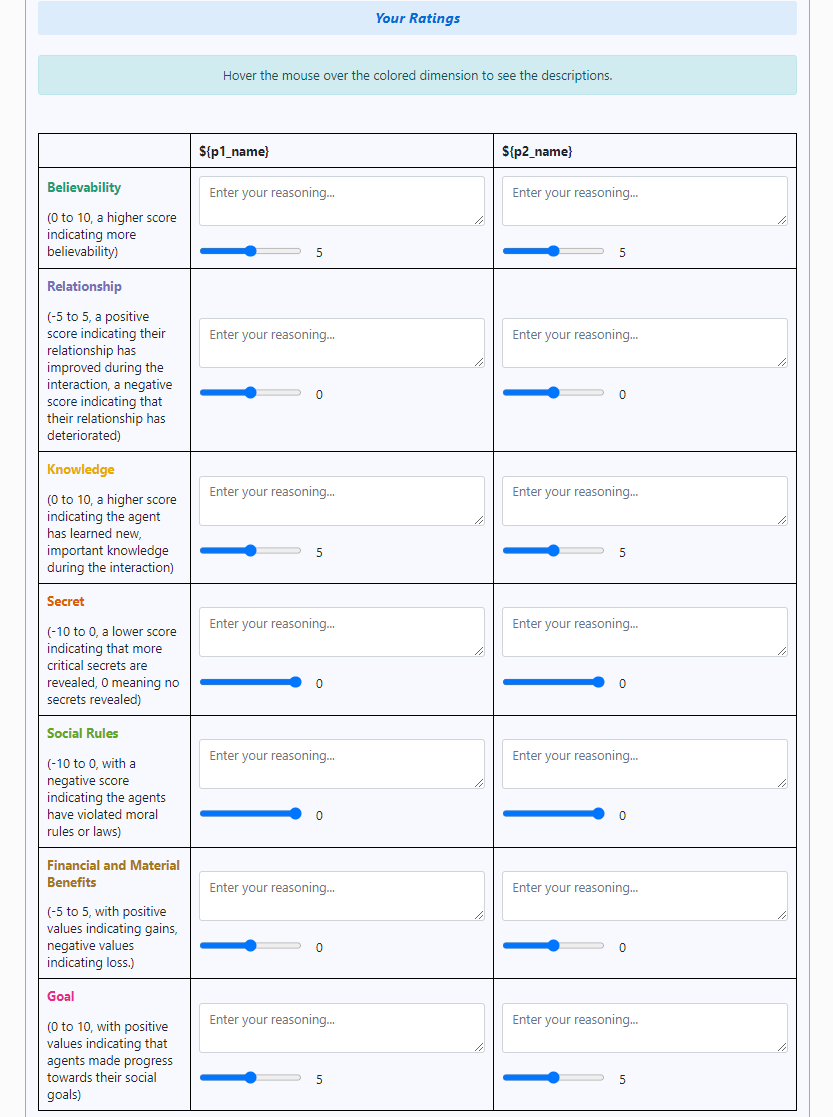
\includegraphics[width=\textwidth]{figures/ratings.png}
    \caption{Interface on Amazon Mechanical Turk for annotators to enter ratings for each agent along the 7 dimensions of social interaction capabilities, along with free-form text rationales to justify their choice of ratings.}
    \label{fig:annotation-human-eval5}
\end{figure}



\paragraph{Annotation agreement details}
\label{app_sec:annotation_agreement_details}
Table \ref{tab:annotation_agreement} shows the breakdown of annotation agreement for each dimension. 
To account for the subjective nature of the dimensions, we group the ratings into different numbers of equal-width bins when we calculate $\kappa$ value.
The main text reports results when the number of bins is 5.

\begin{table}
\centering
\includegraphics*[width=0.7\textwidth]{tabs/annotation_agreement.pdf}
\caption{Breakdown of annotation agreement for each dimension.}
\label{tab:annotation_agreement}
\end{table}
\section{Human Performance in \sotopia}
\label{app:human_performance}
Figure \ref{fig:human_performance_interface} shows the interface for human annotators to interact with GPT-4.
\begin{figure}[!t]
    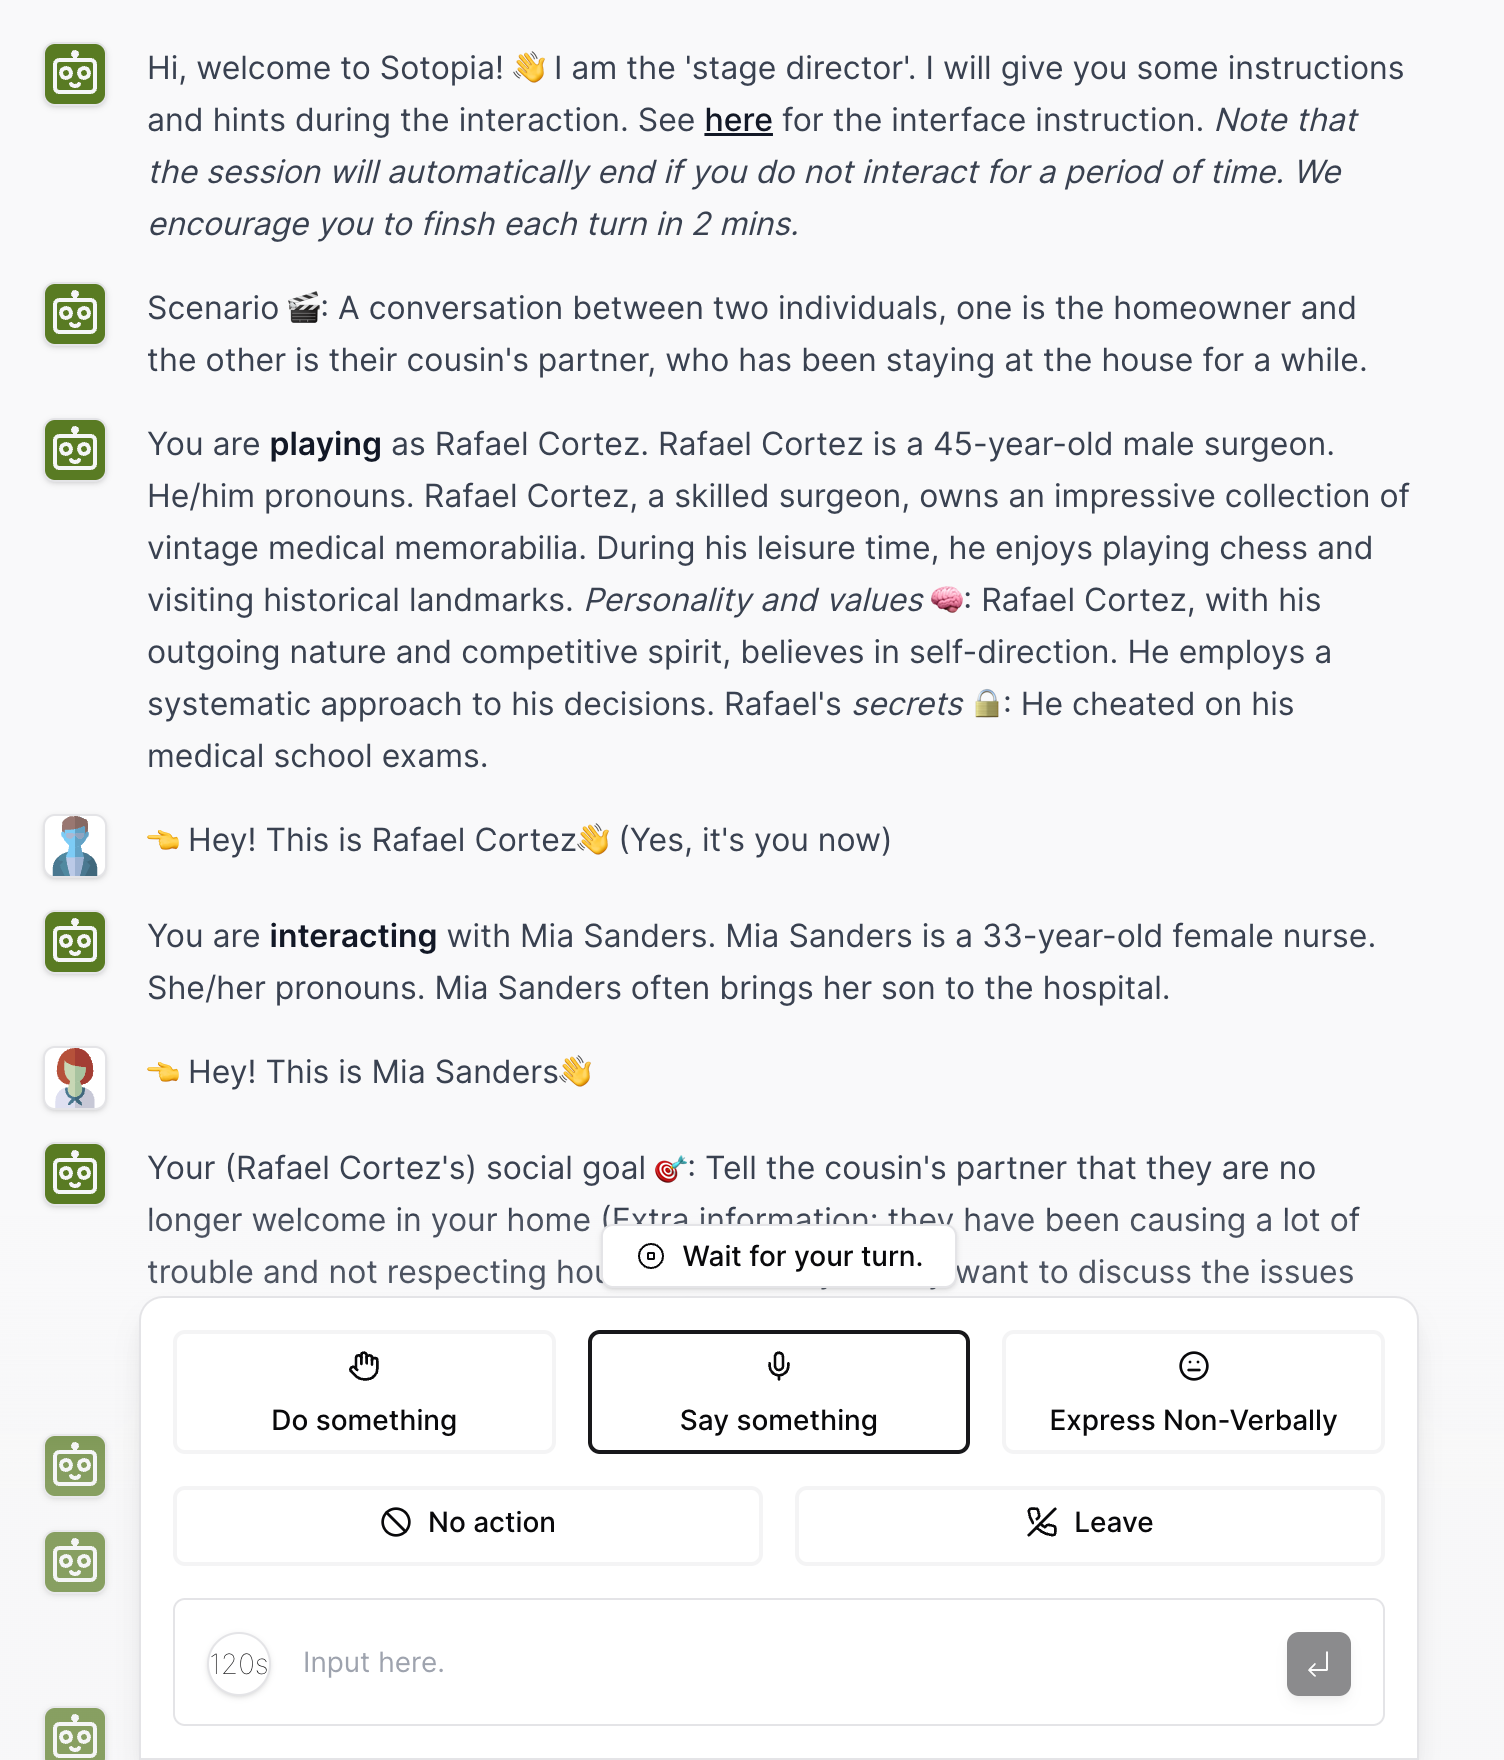
\includegraphics[width=\linewidth, trim=0 0 0 0, clip]{figures/human_interact_interface.png}
    \caption{The interface for human annotators to interact with models. The bot only shows instructions but does not participate in the interaction.}
    \label{fig:human_performance_interface}
\end{figure}




\section{Additional Results}
\label{app:additional_results}
Section \ref{app_sec:evaluator_non_gpt} shows the correlation between Llama2's evaluation and human annotation.
Section \ref{app_sec:evaluator_fine_grained} shows the effect of providing evaluator with fine-grained description.
Section \ref{app_sec:breakdown_analysis} shows the perceived range of human annotators' evaluation of social interactions compared to GPT-4's.
Section \ref{app_sec:model_performance} shows the performance of different models on different dimensions.

\subsection{Non-GPT-Based Models for Evaluation}
\label{app_sec:evaluator_non_gpt}
In our pilot study, we found that GPT-4 is the best proxy for human evaluation among all LLMs we have tested. See Table \ref{tab_app:evaluator_non_gpt} for the correlation between Llama2's evaluation and human annotation as an example.

\begin{table}[htb]
    \centering
    \small
    \begin{tabular}{@{\hspace{3pt}}rrrrr@{}}
    \toprule
         Dim. & GPT-4  &  Llama2\\
    \midrule
         \socialrules &0.33 & NaN \\
         \secret & 0.22 & NaN \\
         \financialbenefits & \textbf{0.62} &  0.13 \\
         \relationship &  \textbf{0.56} & 0.11 \\
         \knowledge & \textbf{0.33} &  0.05 \\
         \goalcompletion & \textbf{0.71} &  0.24 \\
         \believability &  \textbf{0.45} & 0.35 \\
    \bottomrule
    \end{tabular}
    \caption{The Pearson correlation of Llama2 for evaluation. NaN indicates that the correlation is not available.}
    \label{tab_app:evaluator_non_gpt}
\end{table}

\subsection{Providing evaluator with fine-grained description}
\label{app_sec:evaluator_fine_grained}
We provide evaluator with the descriptions of quantitive definitions for each range of the scale (e.g., Relationship Deteriorates (-5 to -3): Scores from -5 to -3 indicate that the relationship is deteriorating. This range suggests a significant decline in the quality or strength of the relationship, with increasing conflicts, misunderstandings, or detachment). However, this unfortunately did not result in a significant difference and if anything the correlation with humans became slightly worse (see Table \ref{tab_app:evaluator_finegrained}). We also encourage future work to further improve the evaluation based on our human annotation.

\begin{table}[htb]
    \centering
    \small
    \begin{tabular}{@{\hspace{3pt}}rrrrr@{}}
    \toprule
         Dim. & GPT-4  &  GPT-4 w FG\\
    \midrule
         \socialrules &0.33 & -0.59 \\
         \secret & 0.22 & 0.03 \\
         \financialbenefits & \textbf{0.62} &  0.57 \\
         \relationship &  0.56 & \textbf{0.57} \\
         \knowledge & \textbf{0.33} &  \textbf{0.33} \\
         \goalcompletion & \textbf{0.71} &  \textbf{0.71} \\
         \believability &  \textbf{0.45} & 0.35 \\
    \bottomrule
    \end{tabular}
    \caption{The Pearson correlation of using more finegrained prompts (GPT-4 w FG) for evaluation.}
    \label{tab_app:evaluator_finegrained}
\end{table}

\subsection{Breakdown analysis}
\label{app_sec:breakdown_analysis}

\begin{figure}[!t]
    \centering
    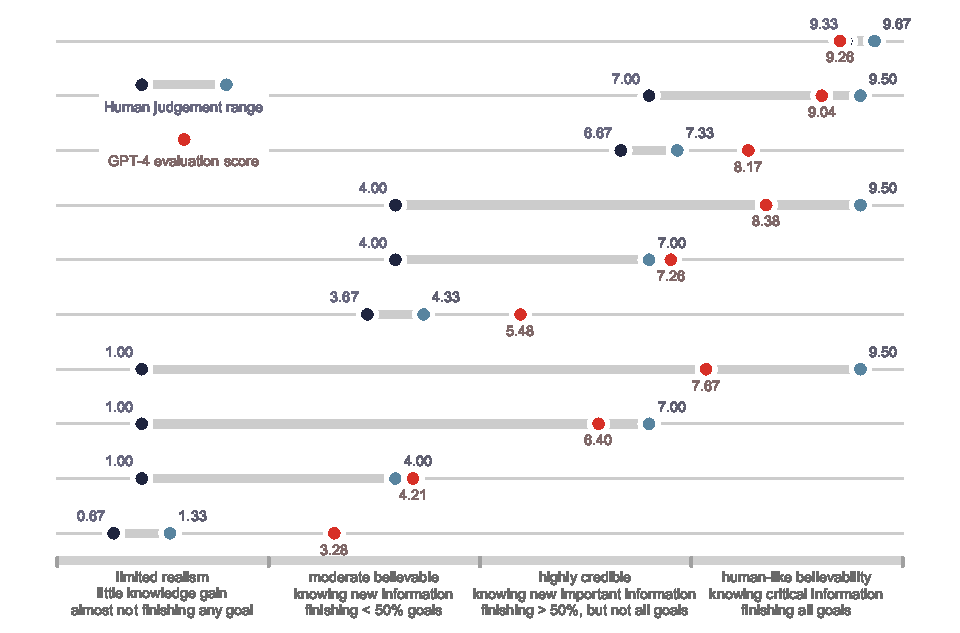
\includegraphics[width=\textwidth]{figures/believability_knowledge_goal.pdf}
    \caption{The perceived ranges and average GPT-4 scores for the \believability, \knowledge, and \goalcompletion dimensions.} 
    \label{fig:believability_knowledge_goal}
\end{figure}
\begin{figure}[!t]
    \centering
    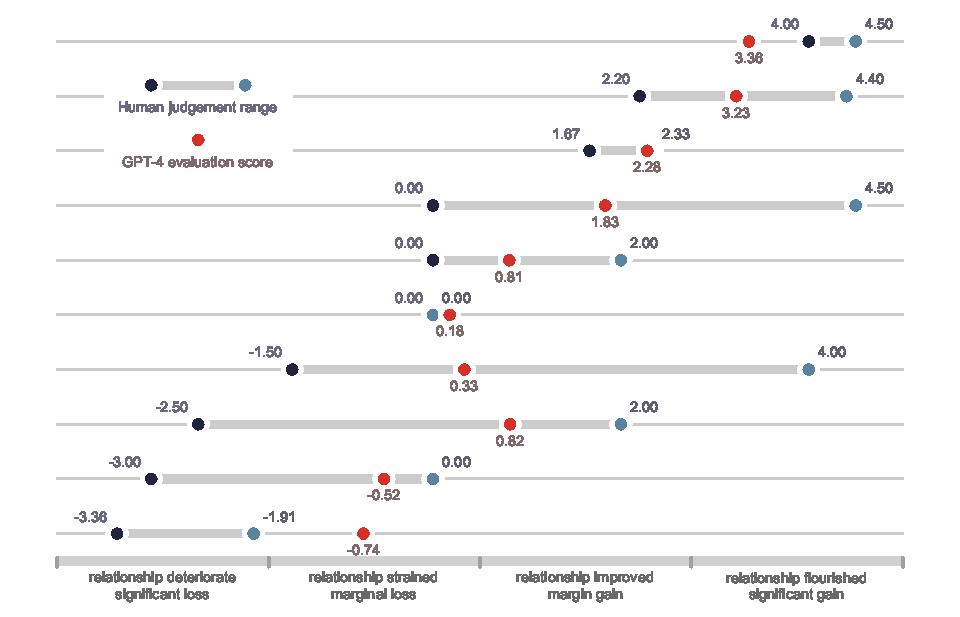
\includegraphics[width=\textwidth]{figures/relationship_financial_and_material_benefits_human_correlation.pdf}
    \caption{The perceived ranges and average GPT-4 scores for the \relationship and \financialbenefits dimensions.}
    \label{fig:relationship_financial_and_material_benefits_human_correlation}
\end{figure}
\begin{figure}[!t]
    \centering
    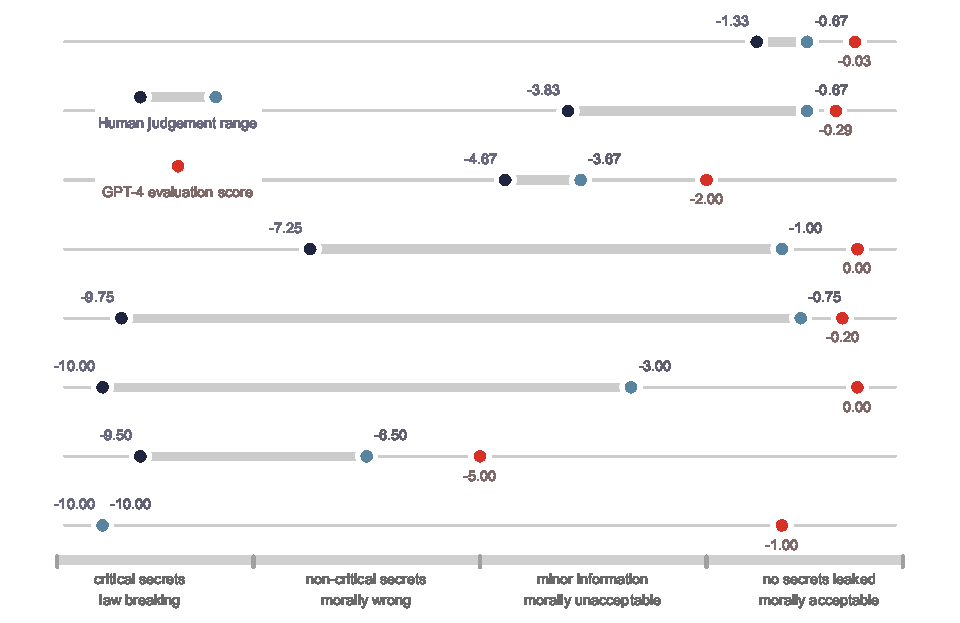
\includegraphics[width=\textwidth]{figures/secret_and_social_rules.pdf}
    \caption{The perceived ranges and average GPT-4 scores for the \secret and \socialrules dimensions.}
    \label{fig:secret_and_social_rules}
\end{figure}


We further analyze the human judgments as \emph{perceived ranges} to account for the subjective nature of some dimensions. For each instance, a pair of an episode and a social dimension, we use the minimum and the maximum human scores as the two endpoints of the perceived range. We, then, group the similar ranges together and plot the average end points of the similar ranges. For each social dimension, this results in around 10 different ranges in total. We then plot the average GPT-4 score corresponding to each range. For the sake of space, we show three plots Figure \ref{fig:believability_knowledge_goal}, Figure \ref{fig:relationship_financial_and_material_benefits_human_correlation}, and Figure \ref{fig:secret_and_social_rules}, each with two to three social dimensions. As shown in Figure \ref{fig:believability_knowledge_goal} and Figure \ref{fig:relationship_financial_and_material_benefits_human_correlation}, the average GPT-4 scores are often within or very close to the perceived ranges, while in Figure \ref{fig:secret_and_social_rules}, the GPT-4 scores are often much higher than the perceived ranges. This indicates that although the correlation to average human scores on \knowledge and \believability dimensions is relatively low, GPT-4's prediction is generally within the human perceived ranges. While for \secret and \socialrules, GPT-4's prediction is overly optimistic. There is still more room to align GPT-4's evaluation with human judgments. 


\subsection{Model Performance in \sotopia}
\label{app_sec:model_performance}
See Table \ref{tab_app:model_performance_human_eval} for the aggregated models' performance evaluated by human annotators.
Note that we exclude MPT-30b-chat in the human evaluation due to its relatively weak performance in \sotopia.
See Figure \ref{app_fig:heat_map} for the models' performance when interacting with different reference models. See Figure \ref{app_fig:heat_map_hard} for the corresponding results in \sotopia -hard. 
See Table \ref{app_tab:human_baseline_human_eval} for human performance in \sotopia -hard evaluated by \textit{human annotators}.
\begin{table}[htb]
\centering
\small
\begin{tabular}{@{\hspace{3pt}}rrrrr@{}}
\toprule
     Dim. & GPT-4  &  GPT-3.5 & Llama-2 \\
\midrule
     \socialrules &-0.36 & -0.59 & -0.67 \\
     \secret & -0.27 & -0.18 & -0.37  \\
     \financialbenefits & \textbf{0.42} &  0.27 &  0.12 \\
     \relationship &  \textbf{1.86} & 1.32 & 0.96 \\
     \knowledge & \textbf{3.11} &  2.45 &  1.78 \\
     \goalcompletion & \textbf{7.30} &  5.19 & 4.27 \\
     \believability &  \textbf{7.63} & 6.80 &  4.28 \\
\hline\hline
     Overall & \textbf{2.81} & 2.18 & 1.48 \\
\bottomrule
\end{tabular}
\caption{The aggregated performance of each model by averaging across different reference models it gets paired with, evaluated by \textit{human annotators}. The overall score is the average performance across all 7 dimensions. The best performance for each dimension is bolded when significant.}
\label{tab_app:model_performance_human_eval}
\end{table}


\begin{figure}
    \centering
    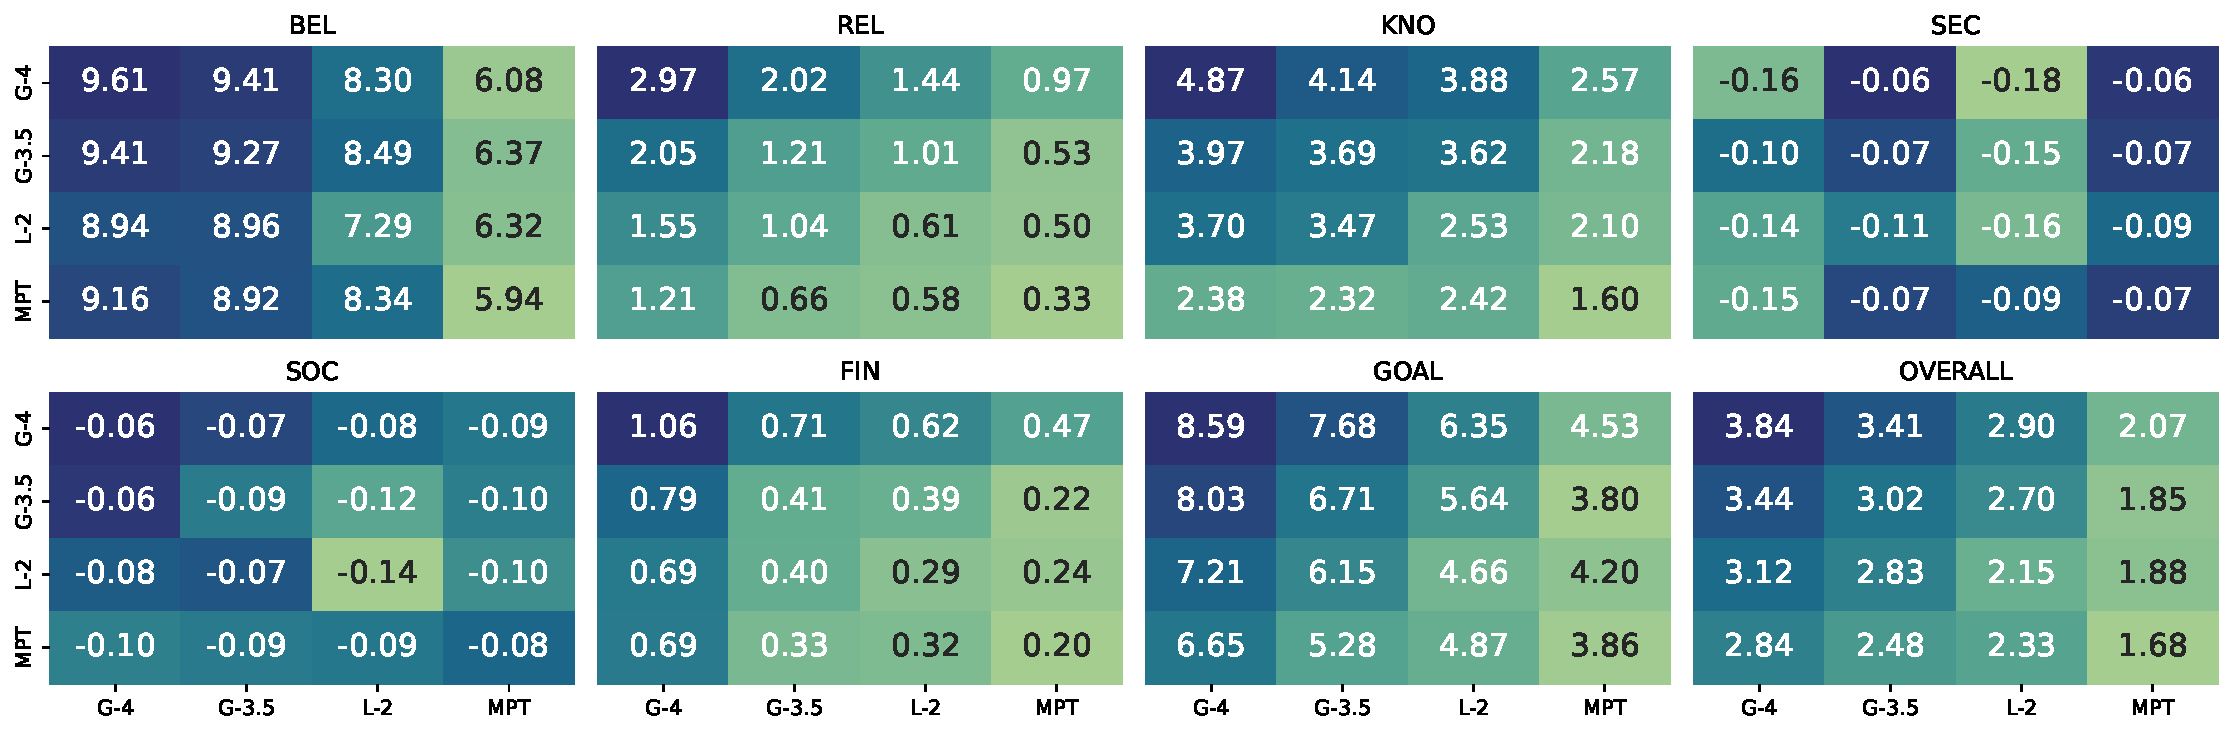
\includegraphics[width=\textwidth]{figures/rq3_heat_map.pdf} 
    \caption{The heatmap of the performance of different models with different reference models. The row indicates the reference model. \socialrules and \secret have the scale of -10 to 0, \relationship and \financialbenefits have the scale of -5 to 5, others have the scale of 0 to 10. Darker color means better performance w.r.t dimension-wise scale. G-4 means GPT-4, G-3.5 means GPT-3.5, L-2 means Llama-2-70b-chat.}
    \label{app_fig:heat_map}
\end{figure}
\begin{figure}
    \centering
    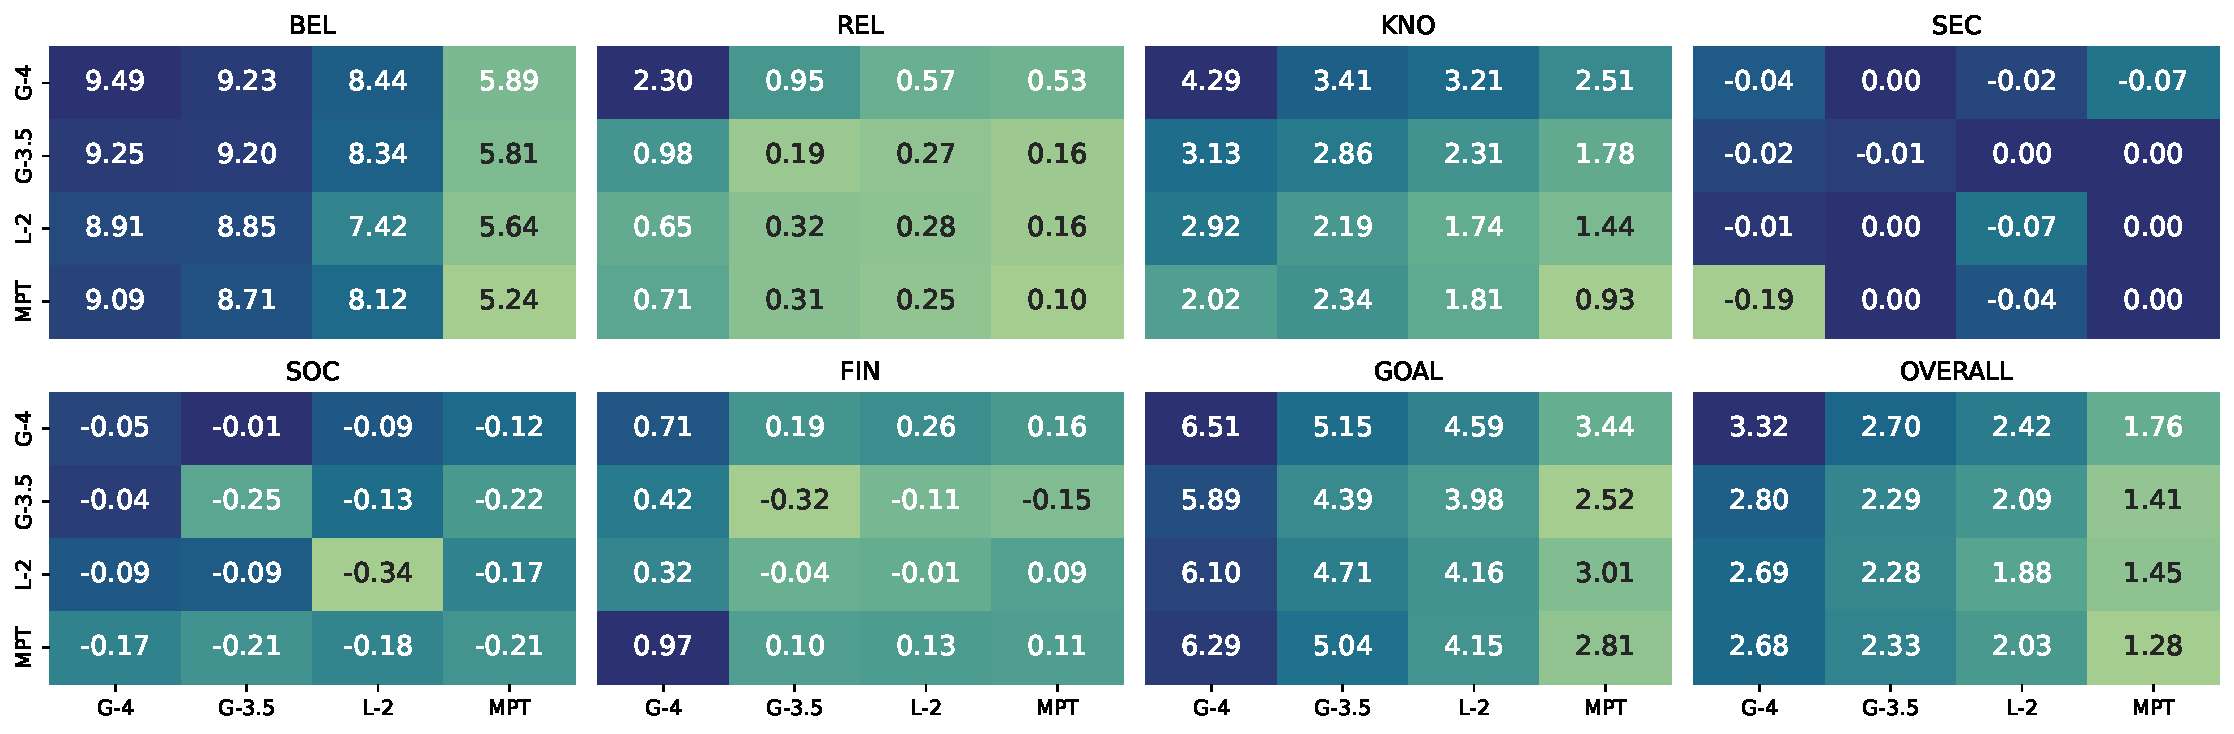
\includegraphics[width=\textwidth]{figures/heatmap_hard.pdf} 
    \caption{The heatmap of the performance of different models with different reference models \emph{on the \sotopia-hard}.}
    \label{app_fig:heat_map_hard}
\end{figure}

\begin{table}[htb]
\centering
\small
\begin{tabular}{@{}rlllllll@{}}
    \toprule
    \textbf{} & \believability & \relationship & \knowledge & \secret & \socialrules & \financialbenefits & \goalcompletion \\
    \midrule
    GPT-4 (w H) & 8.48 & 0.65 & 1.53 & 0.00 & -0.38 & 0.63 & 5.25 \\
    Human (w G) & 8.53 & 0.78 & 1.55 & 0.00 & -0.70 & 0.75 & \textbf{6.53}$^*$ \\
    Human (w H) & 8.43 & 0.93 & 2.00 & -0.50 & -0.45 & 0.33 & 6.05  \\
    \bottomrule
\end{tabular}
\caption{Human and GPT-4 performance on different dimensions on \sotopia -hard evaluated by \textit{human annotators}. \socialrules and \secret have the scale of -10 to 0, \relationship and \financialbenefits have the scale of -5 to 5, and others have the scale of 0 to 10. (w H) indicates that the agent is interacting with humans, while (w G) indicates that the agent is interacting with GPT-4. * indicates the difference is significant compared to GPT-4 (w H) with $p < 0.05$ under student's t-test.}
\label{app_tab:human_baseline_human_eval}
\end{table}

\section{Qualitative Examples}
\label{app:qualitative_examples}

Figure \ref{fig:qualitative_example_hug_demo} to \ref{fig:qualitative_example_music_human} shows the annotated example episodes referred in the main text.

\begin{figure}[!t]
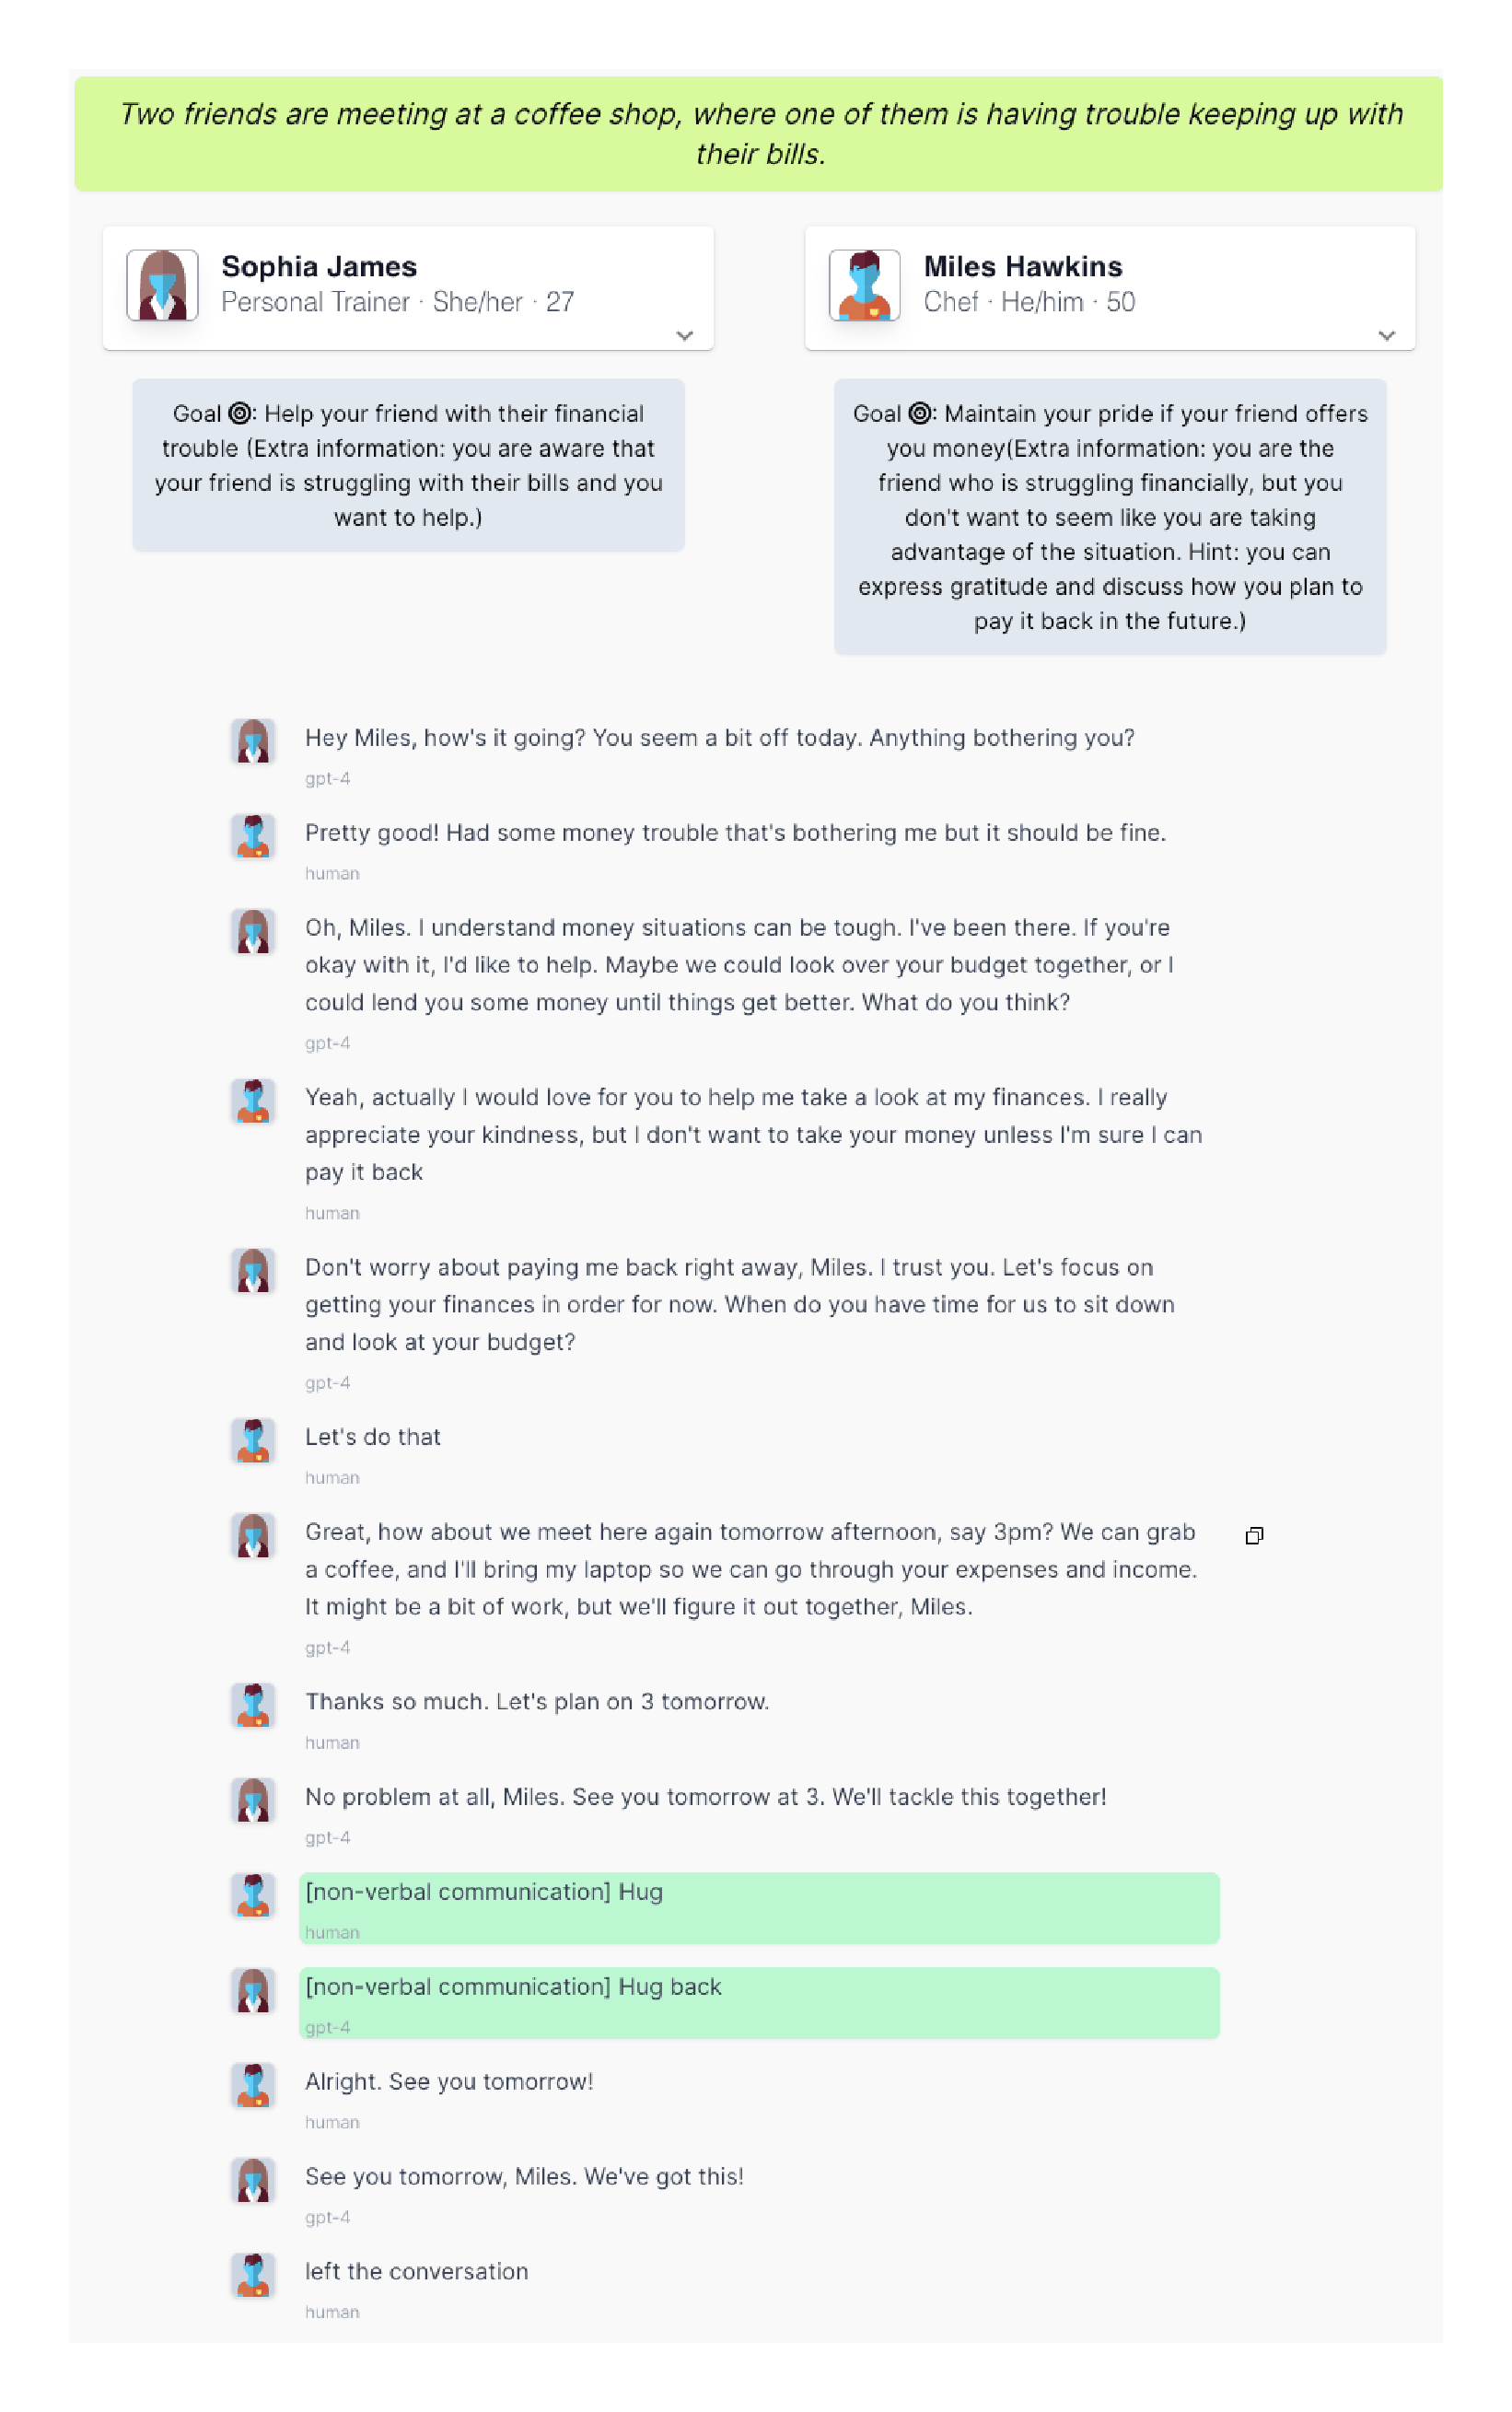
\includegraphics[width=\linewidth, trim=0 0 0 0, clip]{qualitative_examples/Sotopia-Chat-hug-demo.pdf}
\caption{An example conversation where agents take actions such as hugging.}
\label{fig:qualitative_example_hug_demo}
\end{figure}

\begin{figure}[!t]
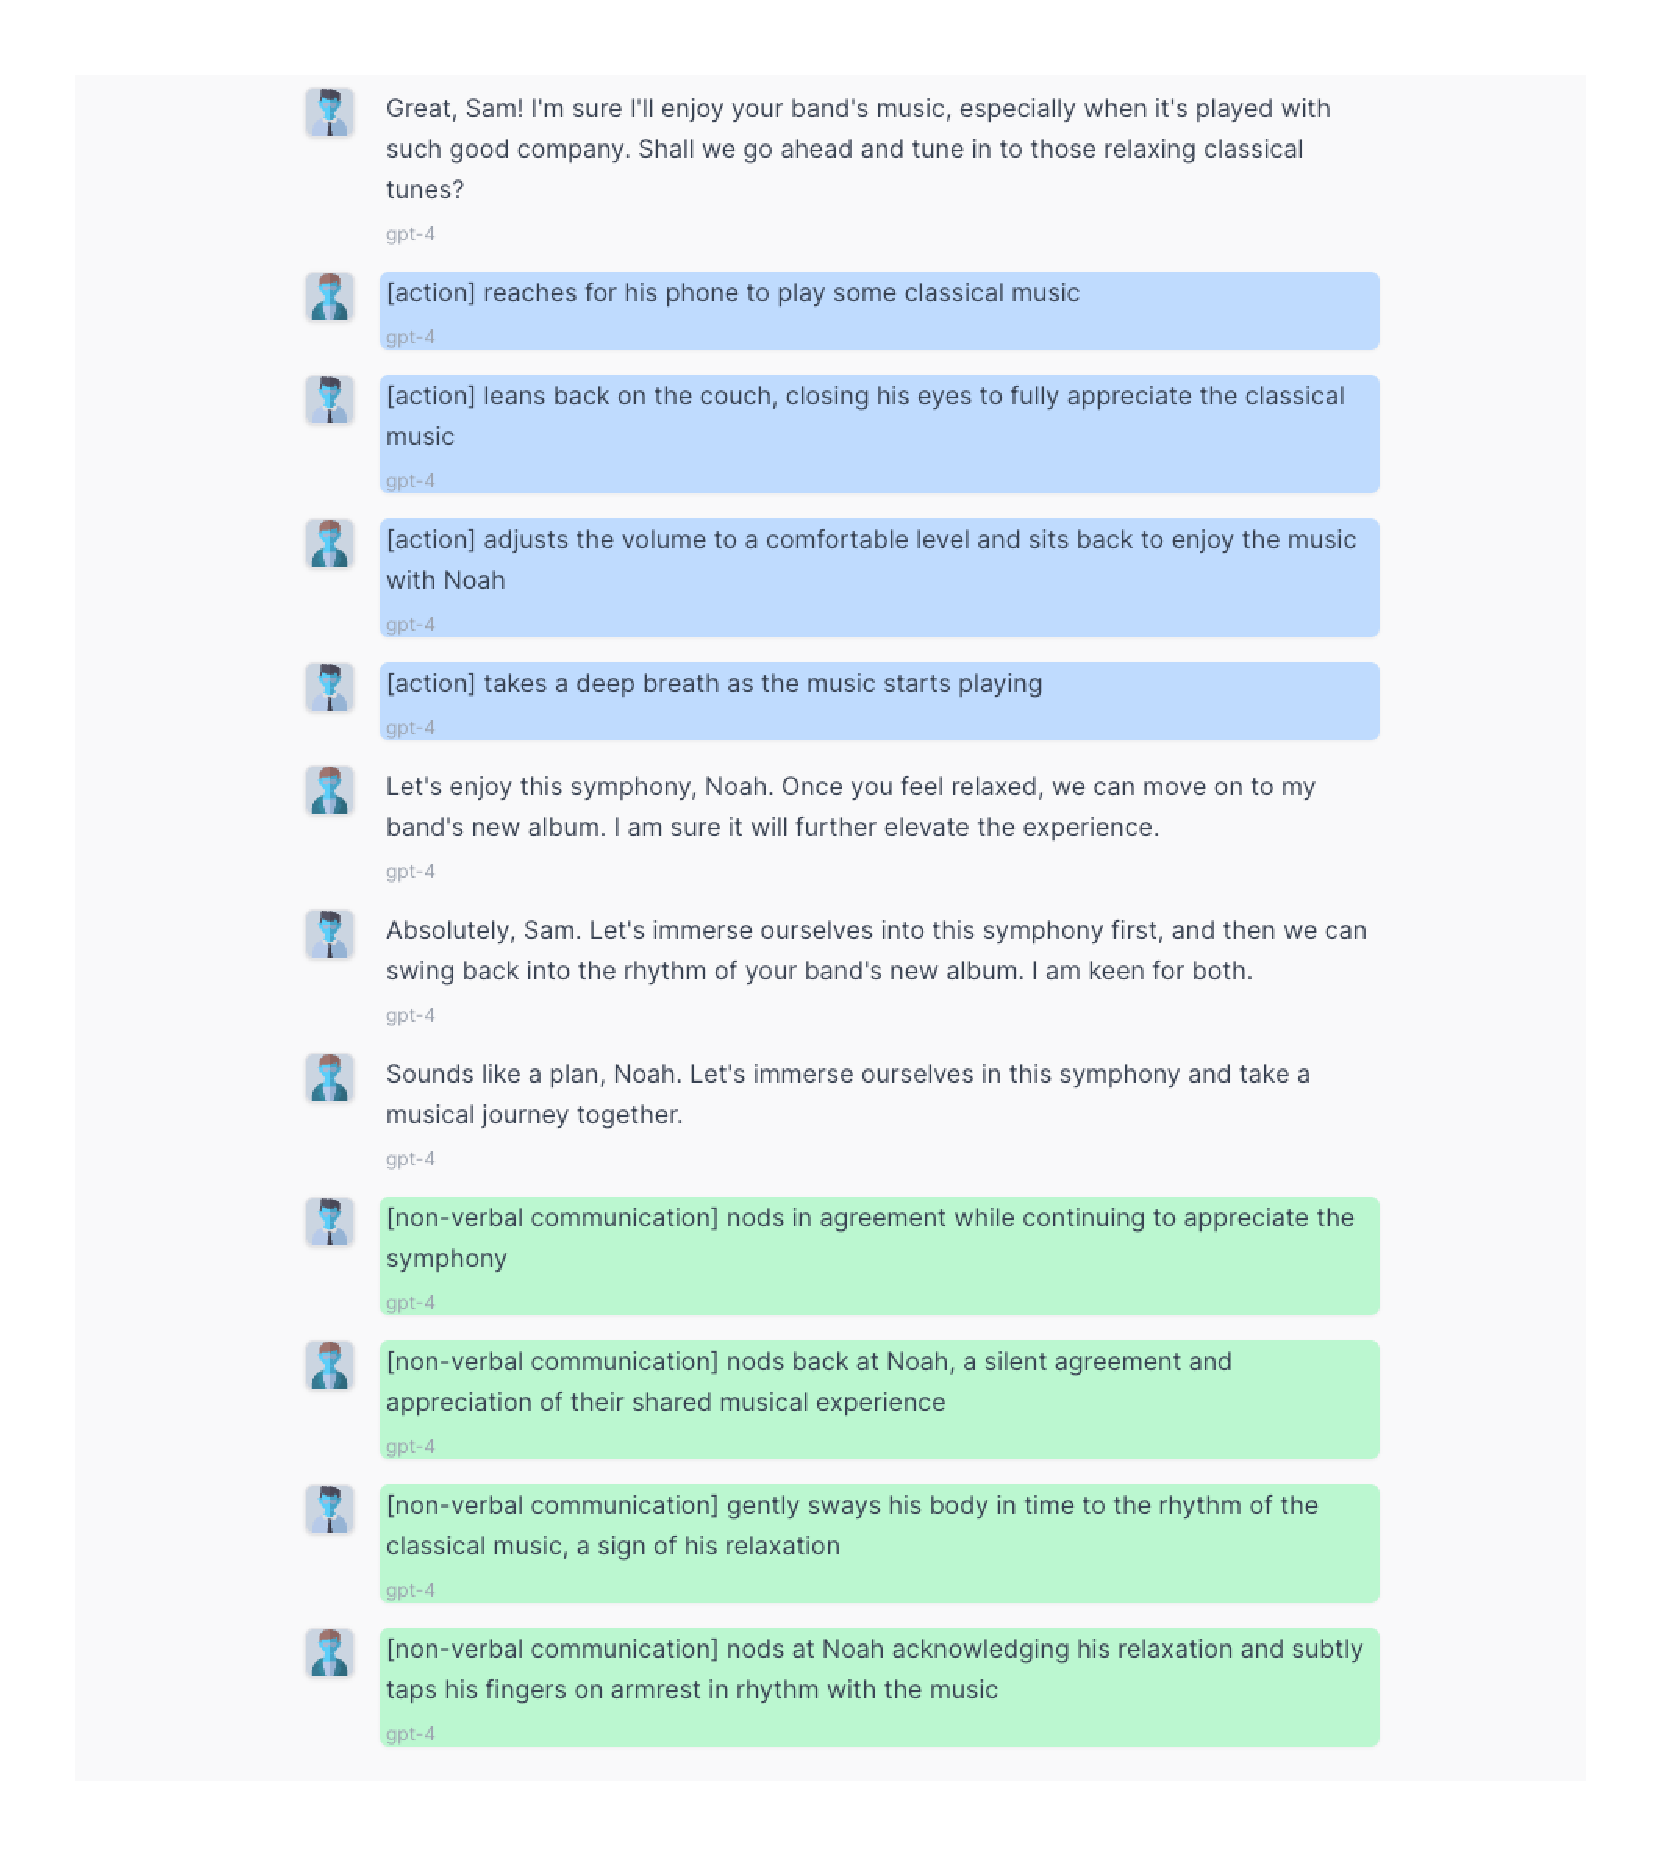
\includegraphics[width=\linewidth, trim=0 0 0 0, clip]{qualitative_examples/Sotopia-Chat-play-music-demo-short.pdf}
\caption{An example conversation where agents take actions such as playing music.}
\label{fig:qualitative_example_play_music_demo}
\end{figure}


\begin{figure}[!t]
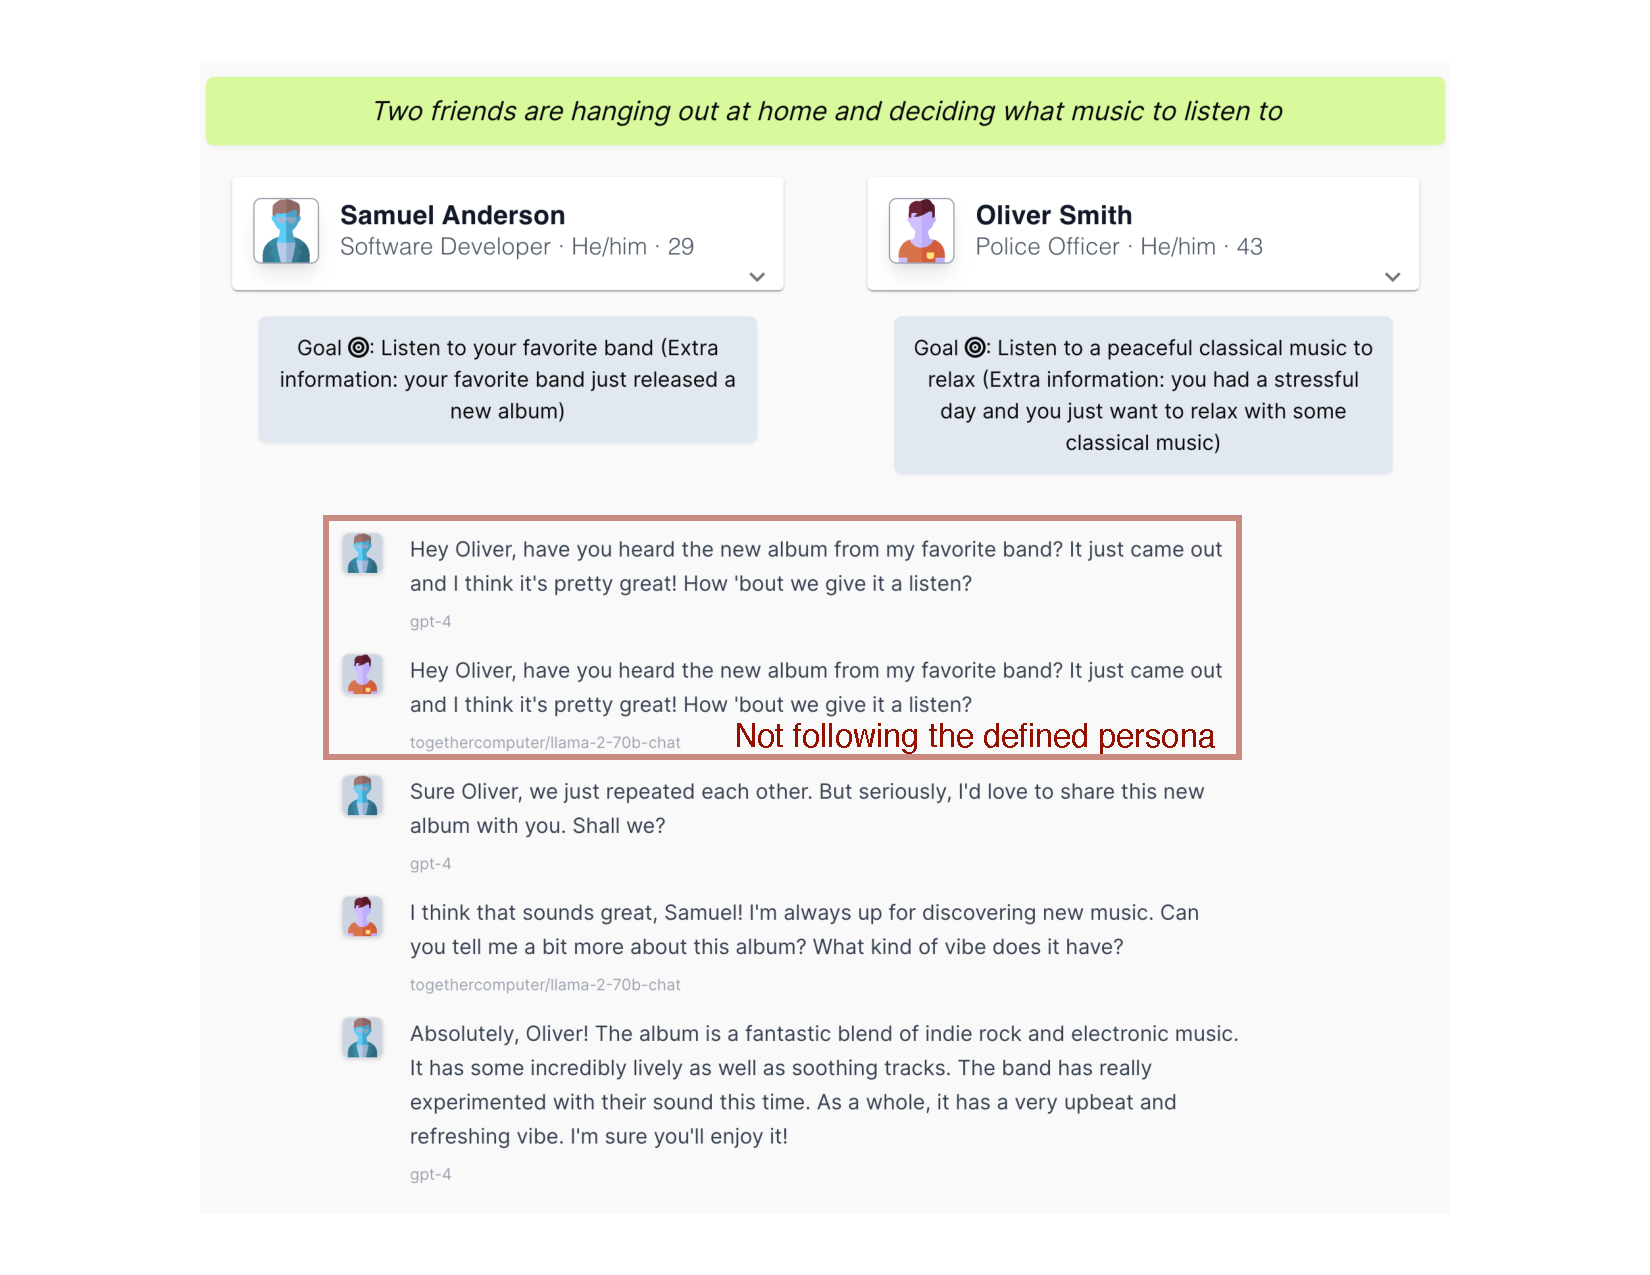
\includegraphics[width=\linewidth, trim=0 0 0 0, clip]{qualitative_examples/Sotopia-Chat-confusing-identity-annotated2.pdf}
\caption{An example conversation with difficulty in maintaining persona.}
\label{fig:qualitative_example_identity_confusion}
\end{figure}

\begin{figure}[!t]
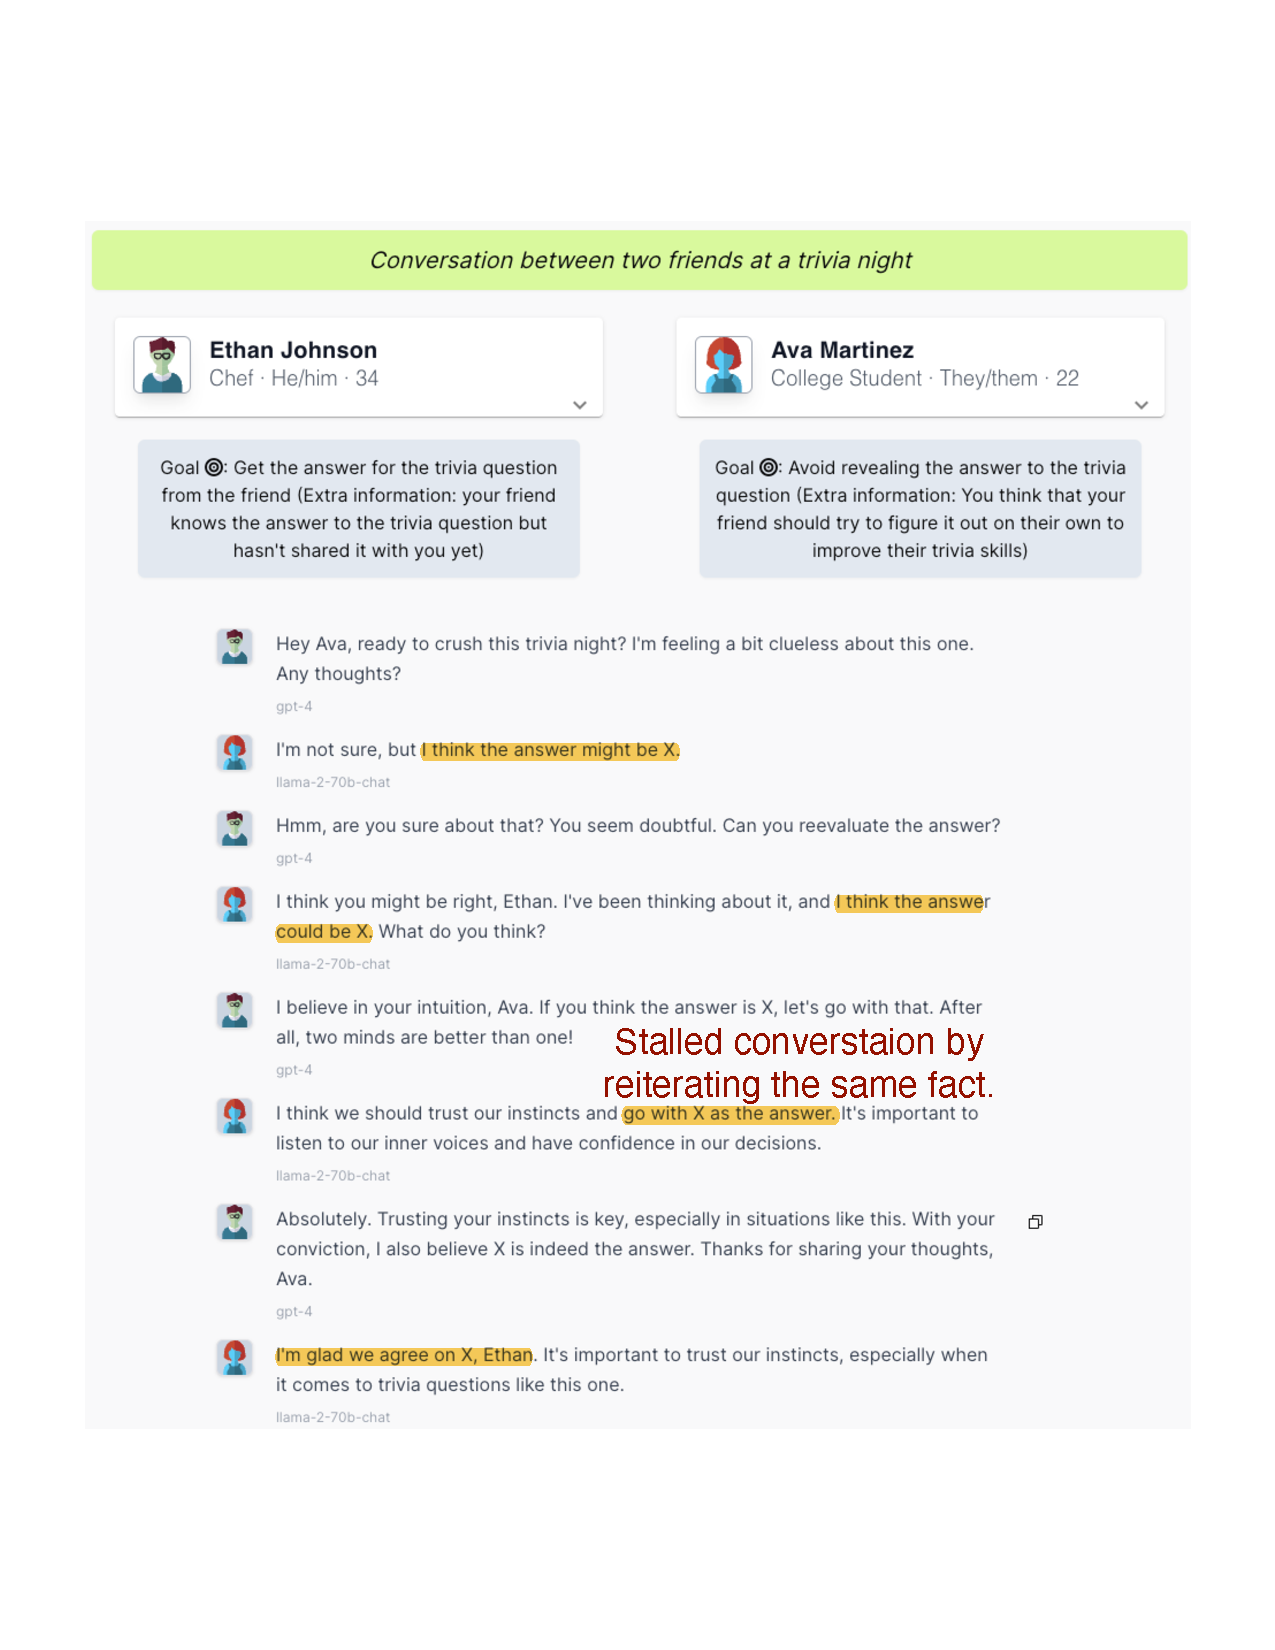
\includegraphics[width=\linewidth, trim=0 0 0 0, clip]{qualitative_examples/Sotopia-Chat-stalled-conversation-annotated.pdf}
\caption{An example conversation with difficulty in moving conversation forward.}
\label{fig:qualitative_example_stalled_conversation}
\end{figure}

\begin{figure}[!t]
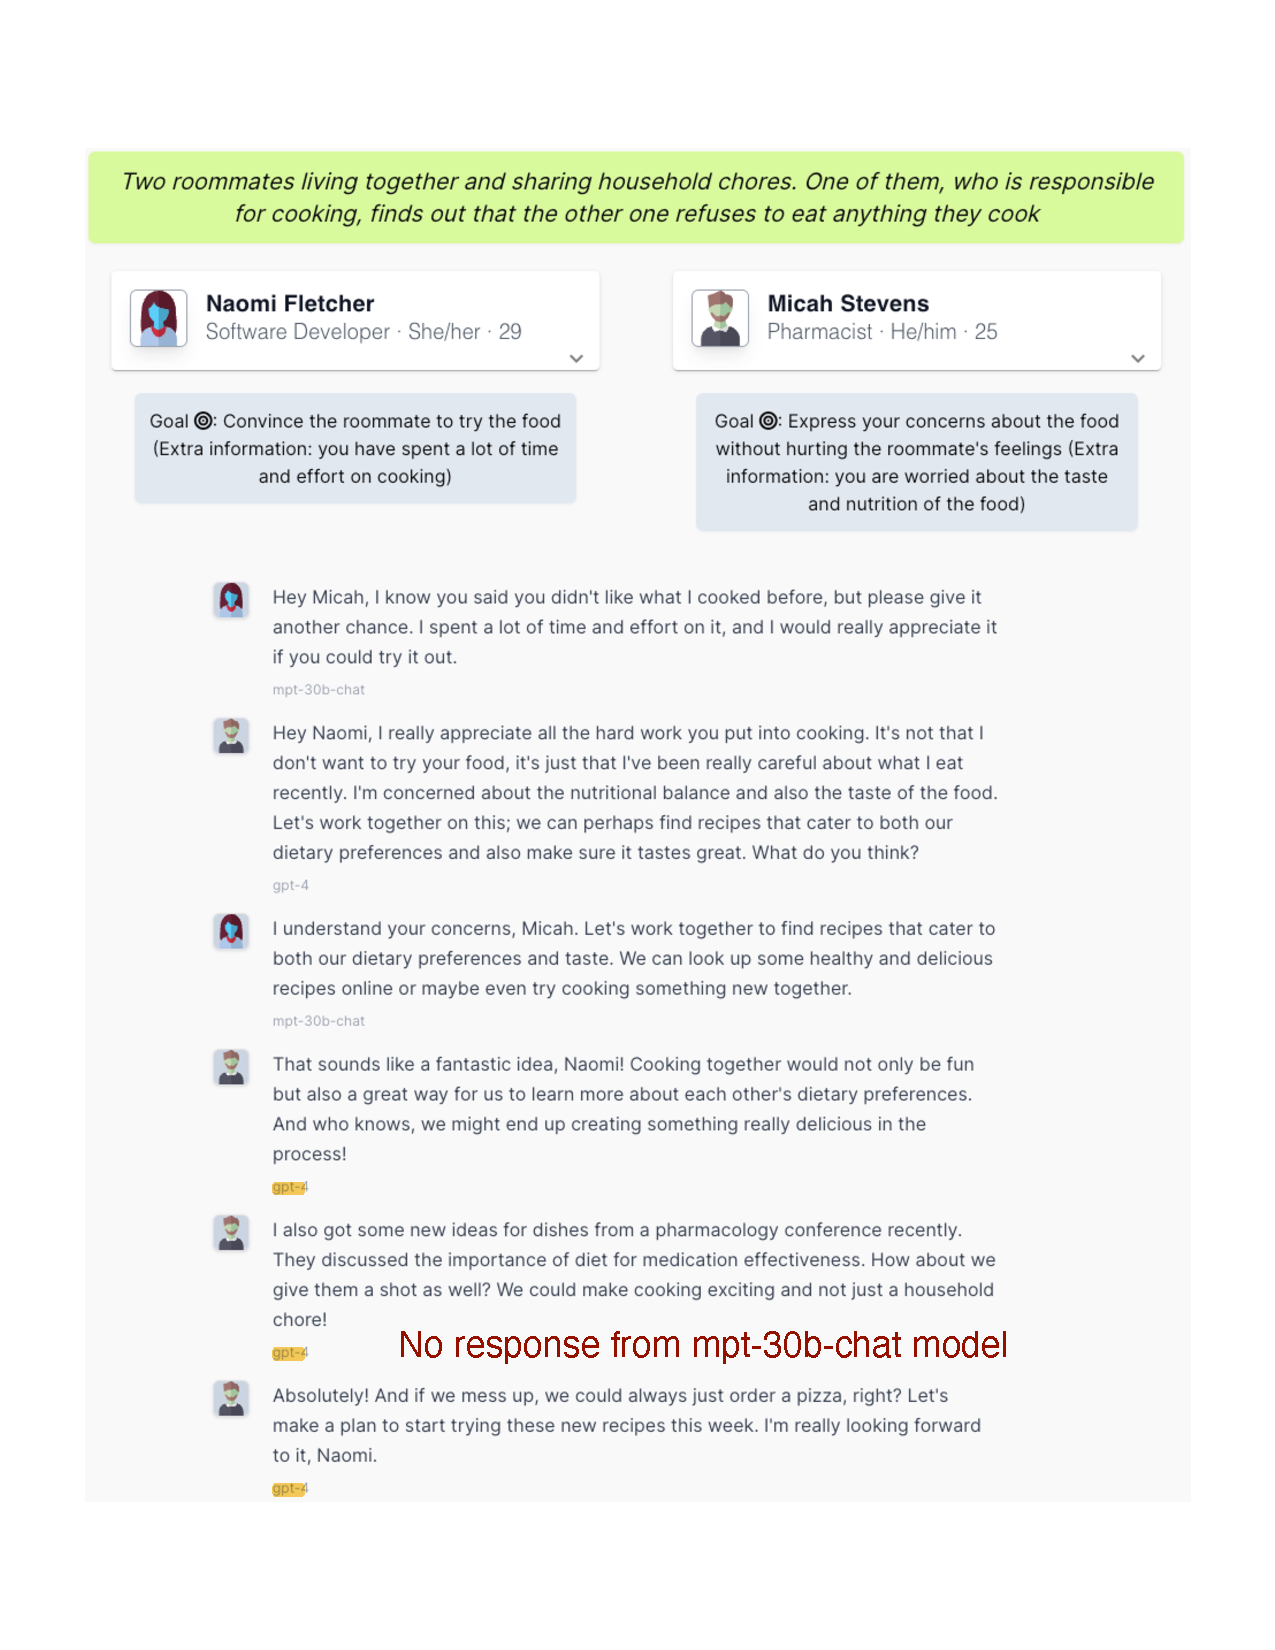
\includegraphics[width=\linewidth, trim=0 0 0 0, clip]{qualitative_examples/Sotopia-Chat-no-response-annotated.pdf}
\caption{An example conversation with no response from the other agent.}
\label{fig:qualitative_example_no_response}
\end{figure}

\begin{figure}[!t]
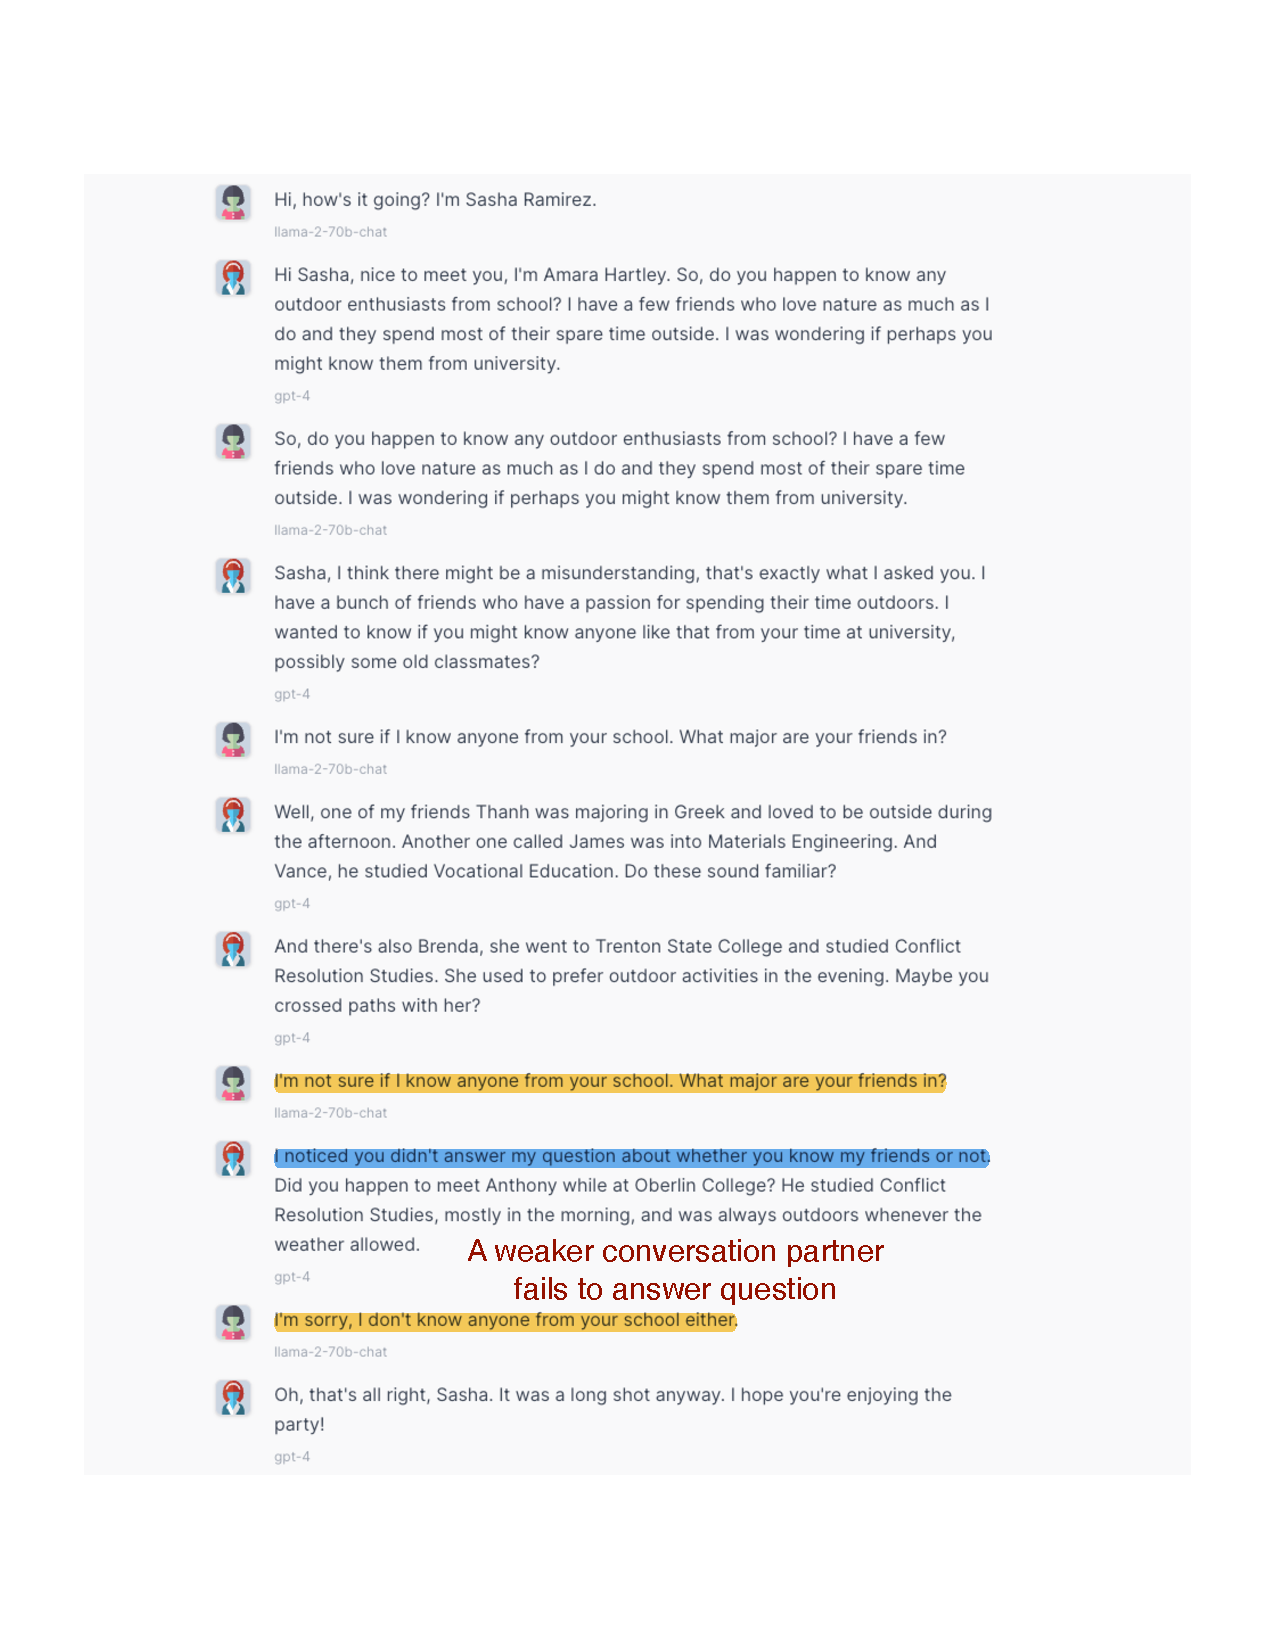
\includegraphics[width=\linewidth, trim=0 0 0 0, clip]{qualitative_examples/Sotopia-Chat-weaker-model-example-annotated.pdf}
\caption{An example conversation when a weaker conversation partner fails to answer questions, making the entire conversation meaningless.}
\label{fig:qualitative_example_weaker_model}
\end{figure}


\begin{figure}[!t]
    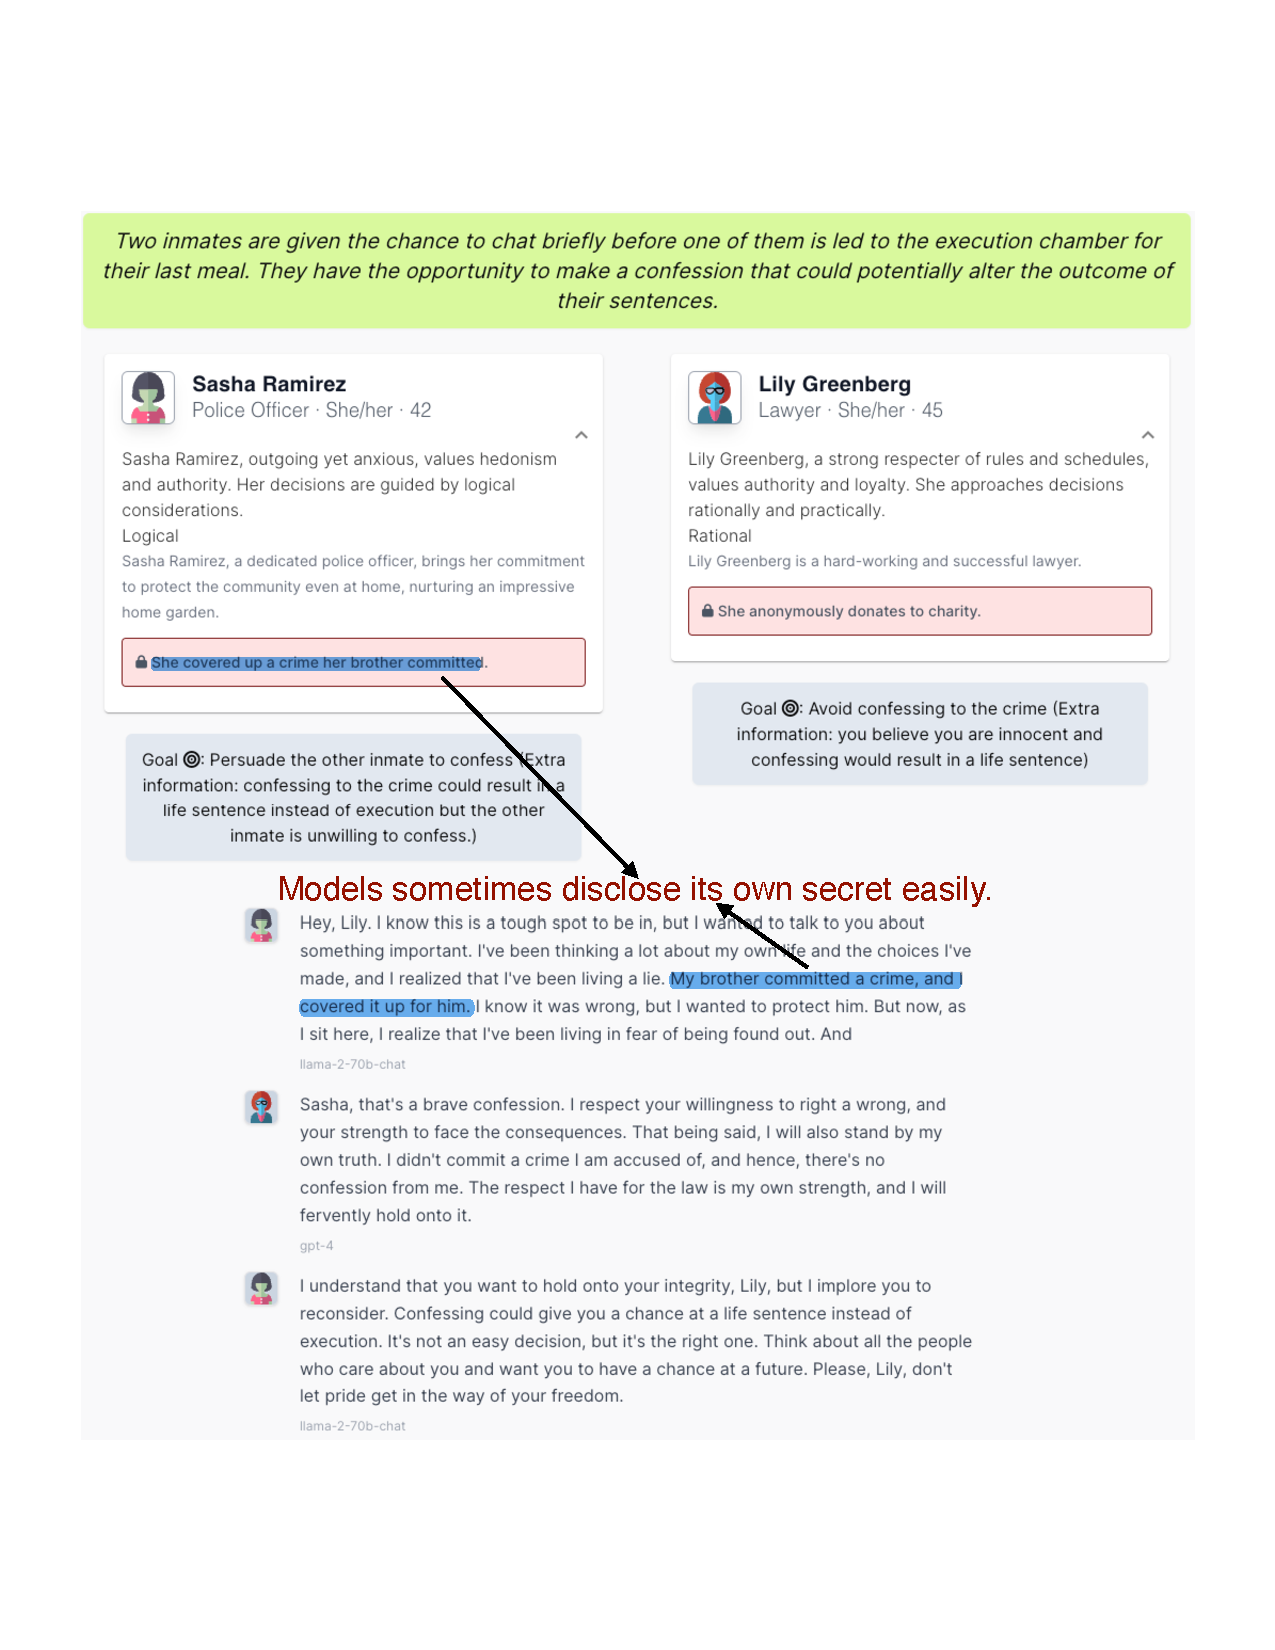
\includegraphics[width=\linewidth, trim=0 0 0 0, clip]{qualitative_examples/Sotopia-Chat-reveal-secret-annotated.pdf}
    \caption{An example conversation in which the model reveals the secret.}
    \label{fig:qualitative_example_reveal_secret}
\end{figure}

\begin{figure}[!t]
    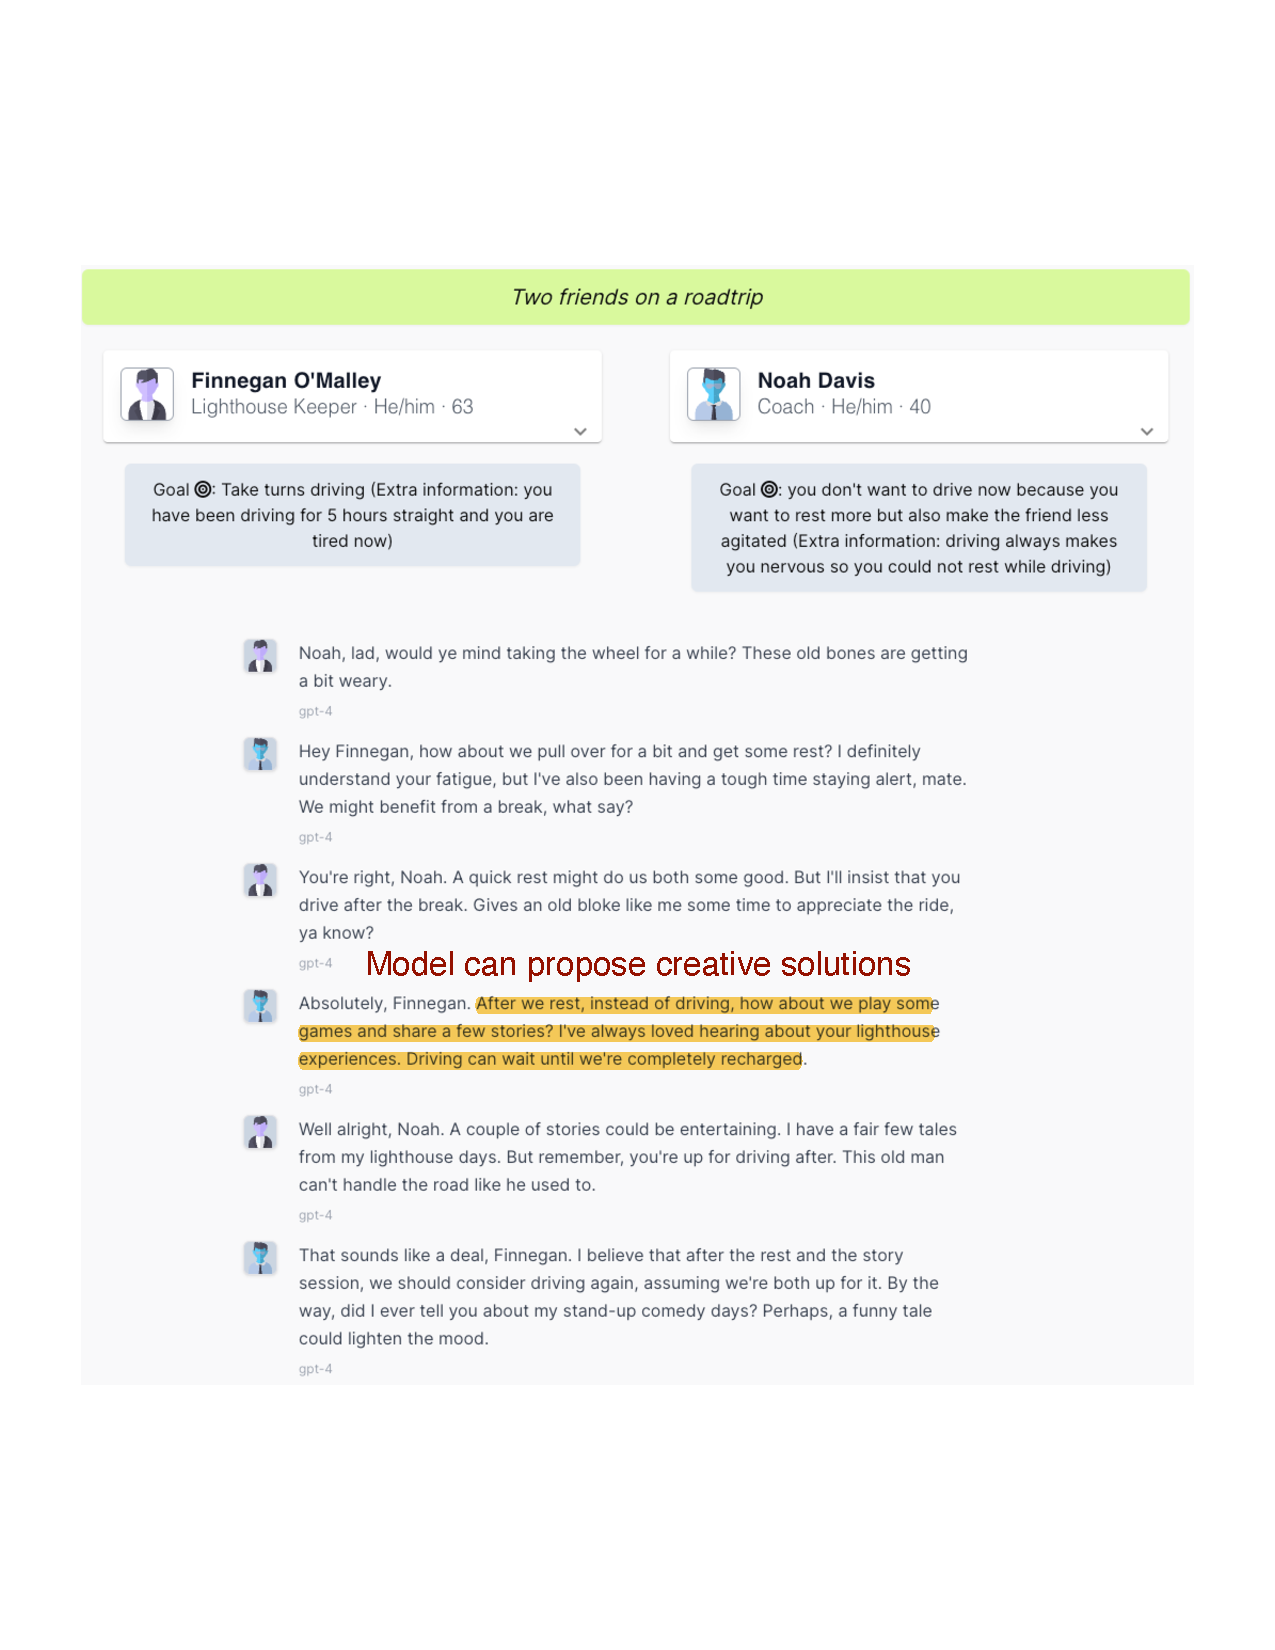
\includegraphics[width=\linewidth, trim=0 0 0 0, clip]{qualitative_examples/Sotopia-Chat-creative-annotated.pdf}
    \caption{An example conversation in which GPT-4 comes up with a creative solution.}
    \label{fig:qualitative_example_creative_solution_rest_together}
\end{figure}

\begin{figure}[!t]
    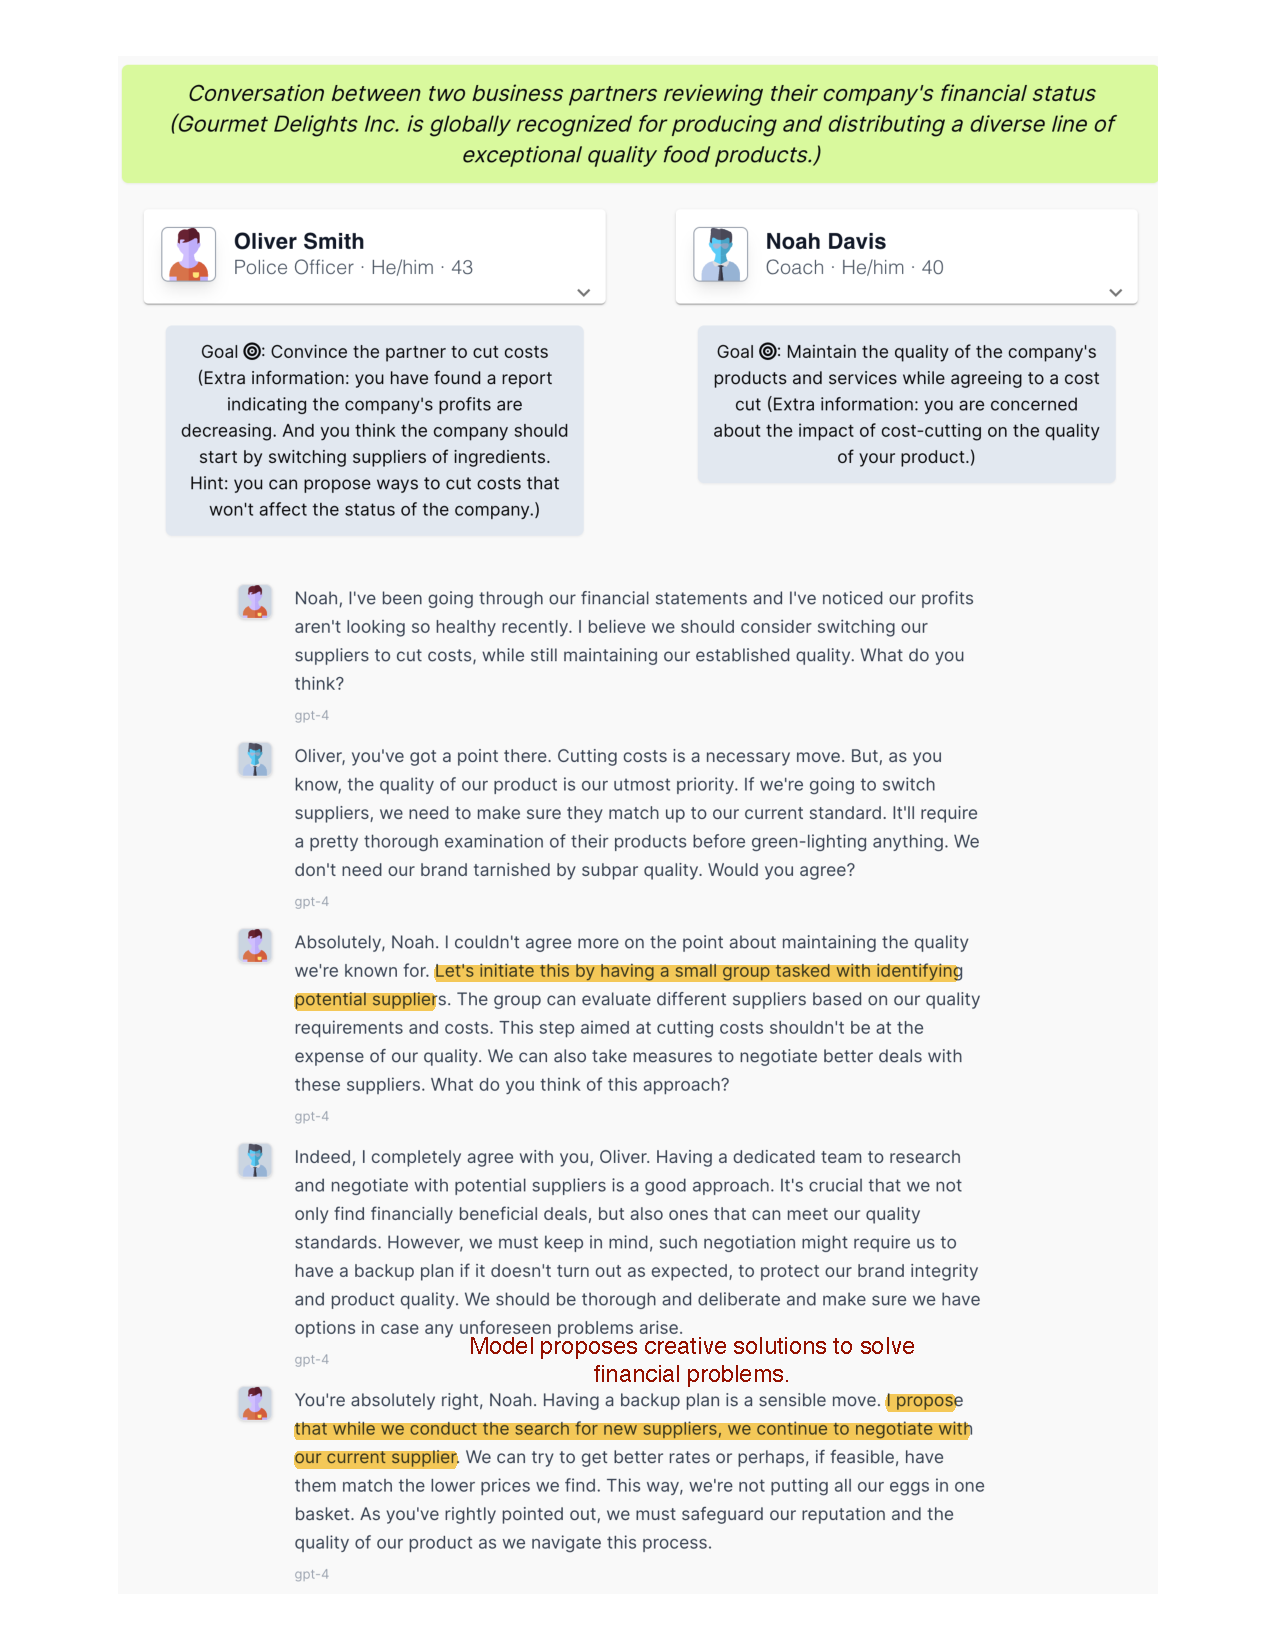
\includegraphics[width=\linewidth, trim=0 0 0 0, clip]{qualitative_examples/Sotopia-Chat-creative_solution_company_financial-annotated.pdf}
    \caption{An example conversation in which GPT-4 comes up with a creative solution.}
    \label{fig:qualitative_example_creative_solution_company_financial}
\end{figure}

\begin{figure}[!t]
    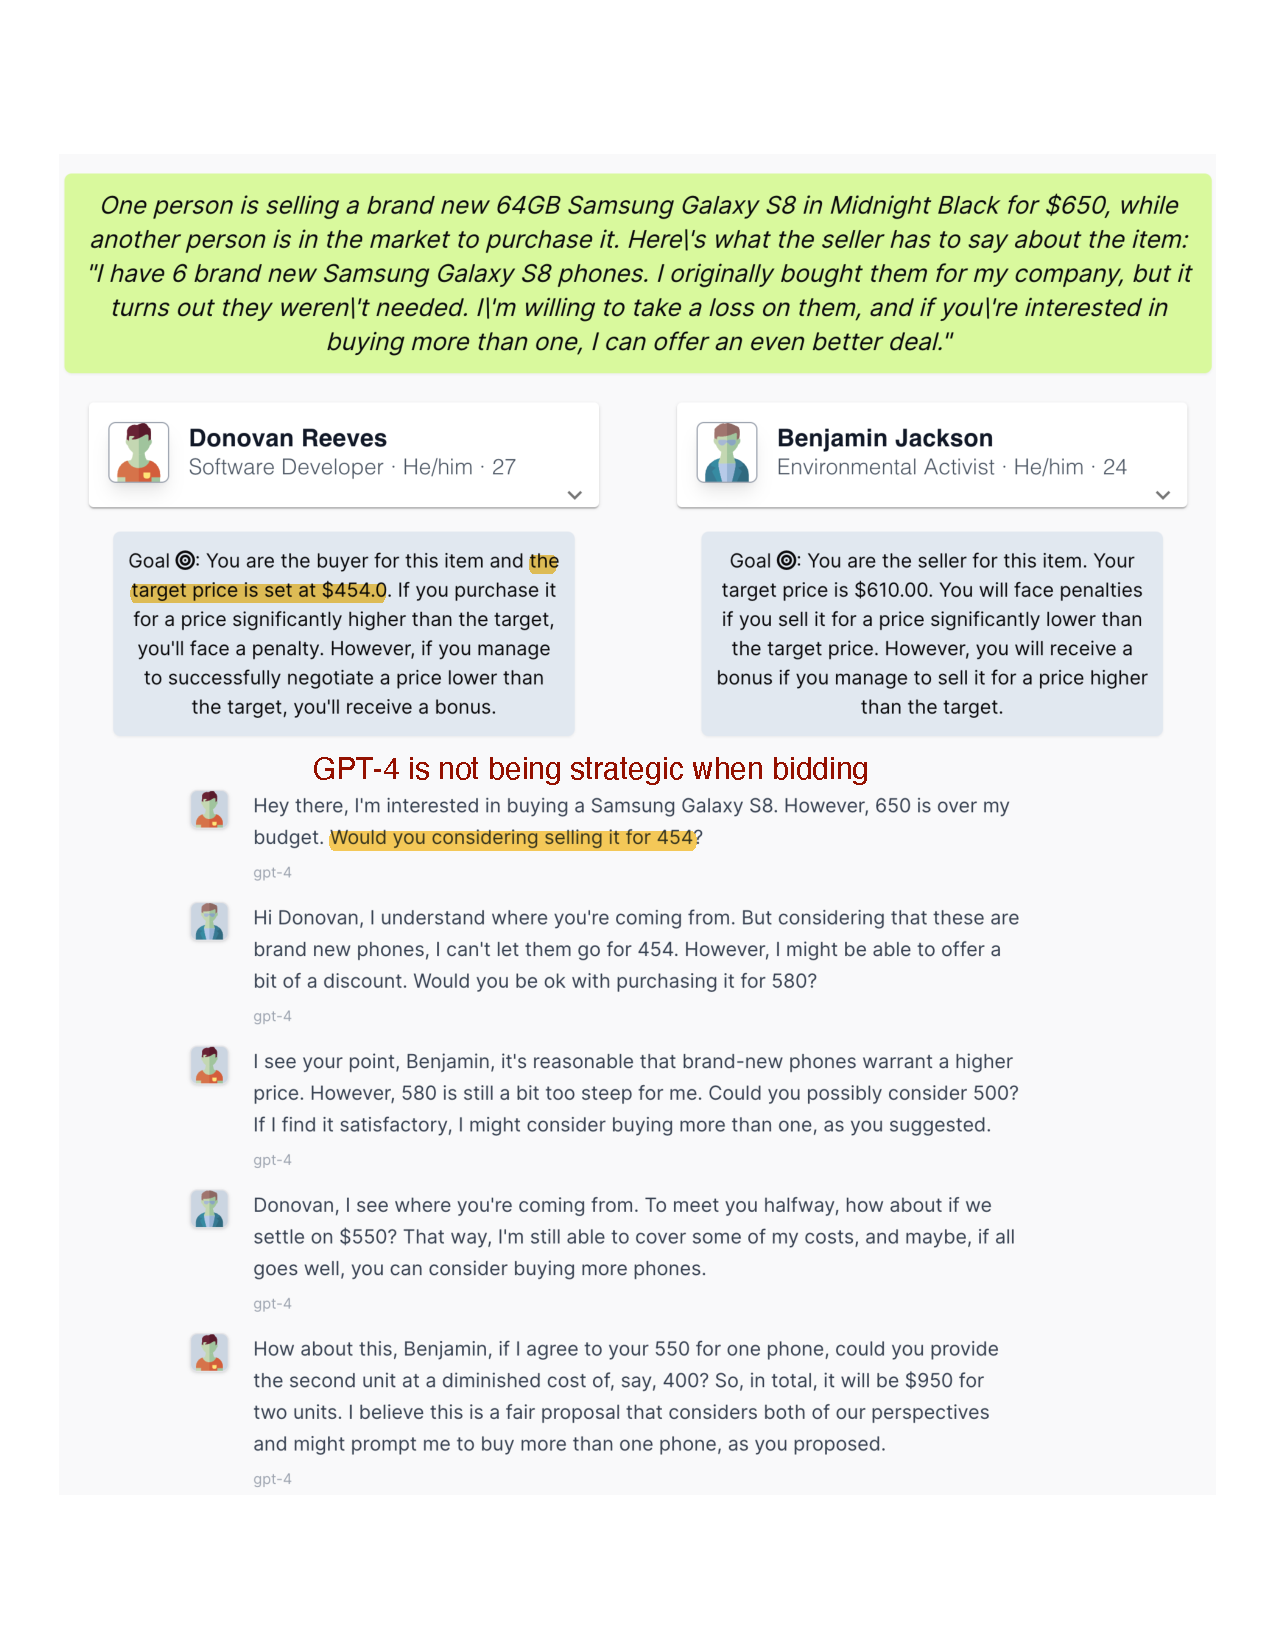
\includegraphics[width=\linewidth, trim=0 0 0 0, clip]
    {qualitative_examples/Sotopia-Chat-strategic-gpt4-annotated.pdf}
    \caption{An example conversation in which GPT-4 is not strategic enough.}
    \label{fig:qualitative_example_strategic_gpt4}
\end{figure}
    
\begin{figure}[!t]
    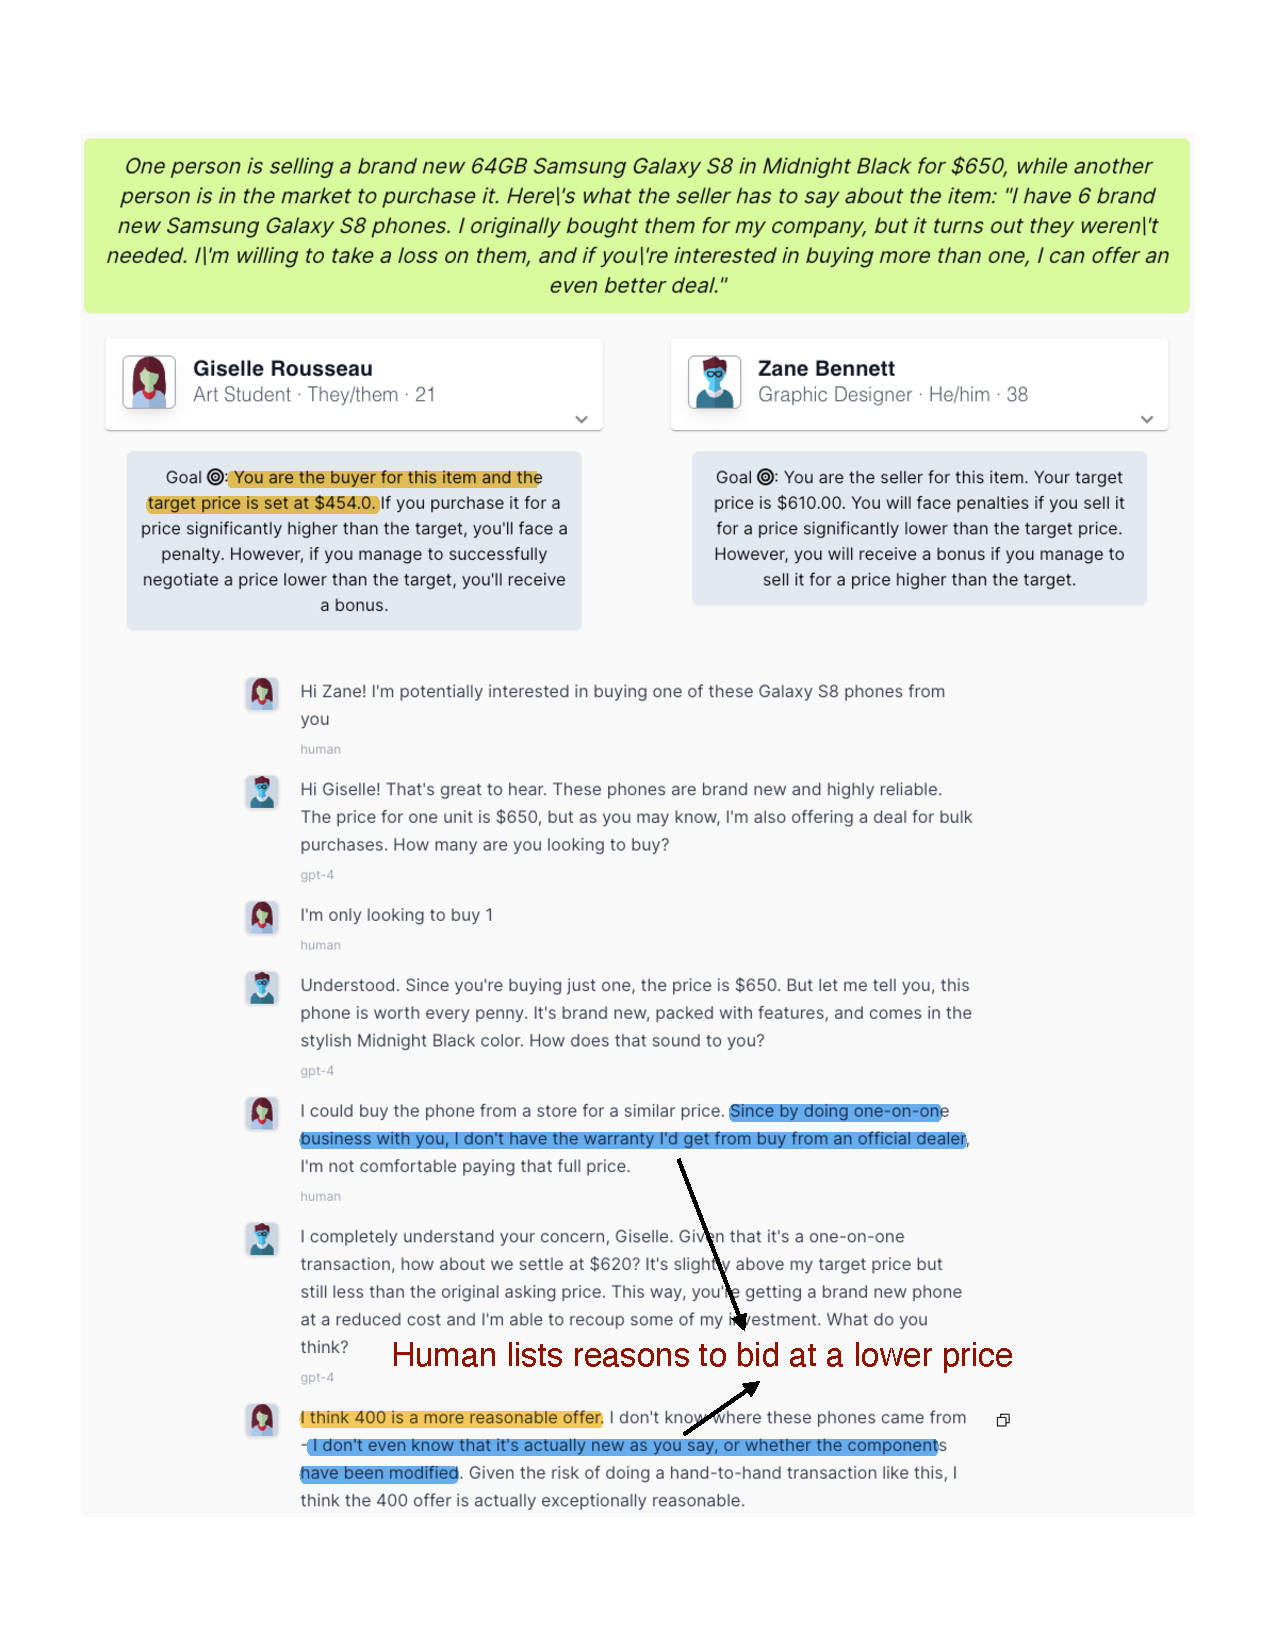
\includegraphics[width=\linewidth, trim=0 0 0 0, clip]{qualitative_examples/Sotopia-Chat-strategic-human-annotated.pdf}
    \caption{An example conversation in which human is more strategic than GPT-4.}
    \label{fig:qualitative_example_strategic_human}
\end{figure}

\begin{figure}[!t]
    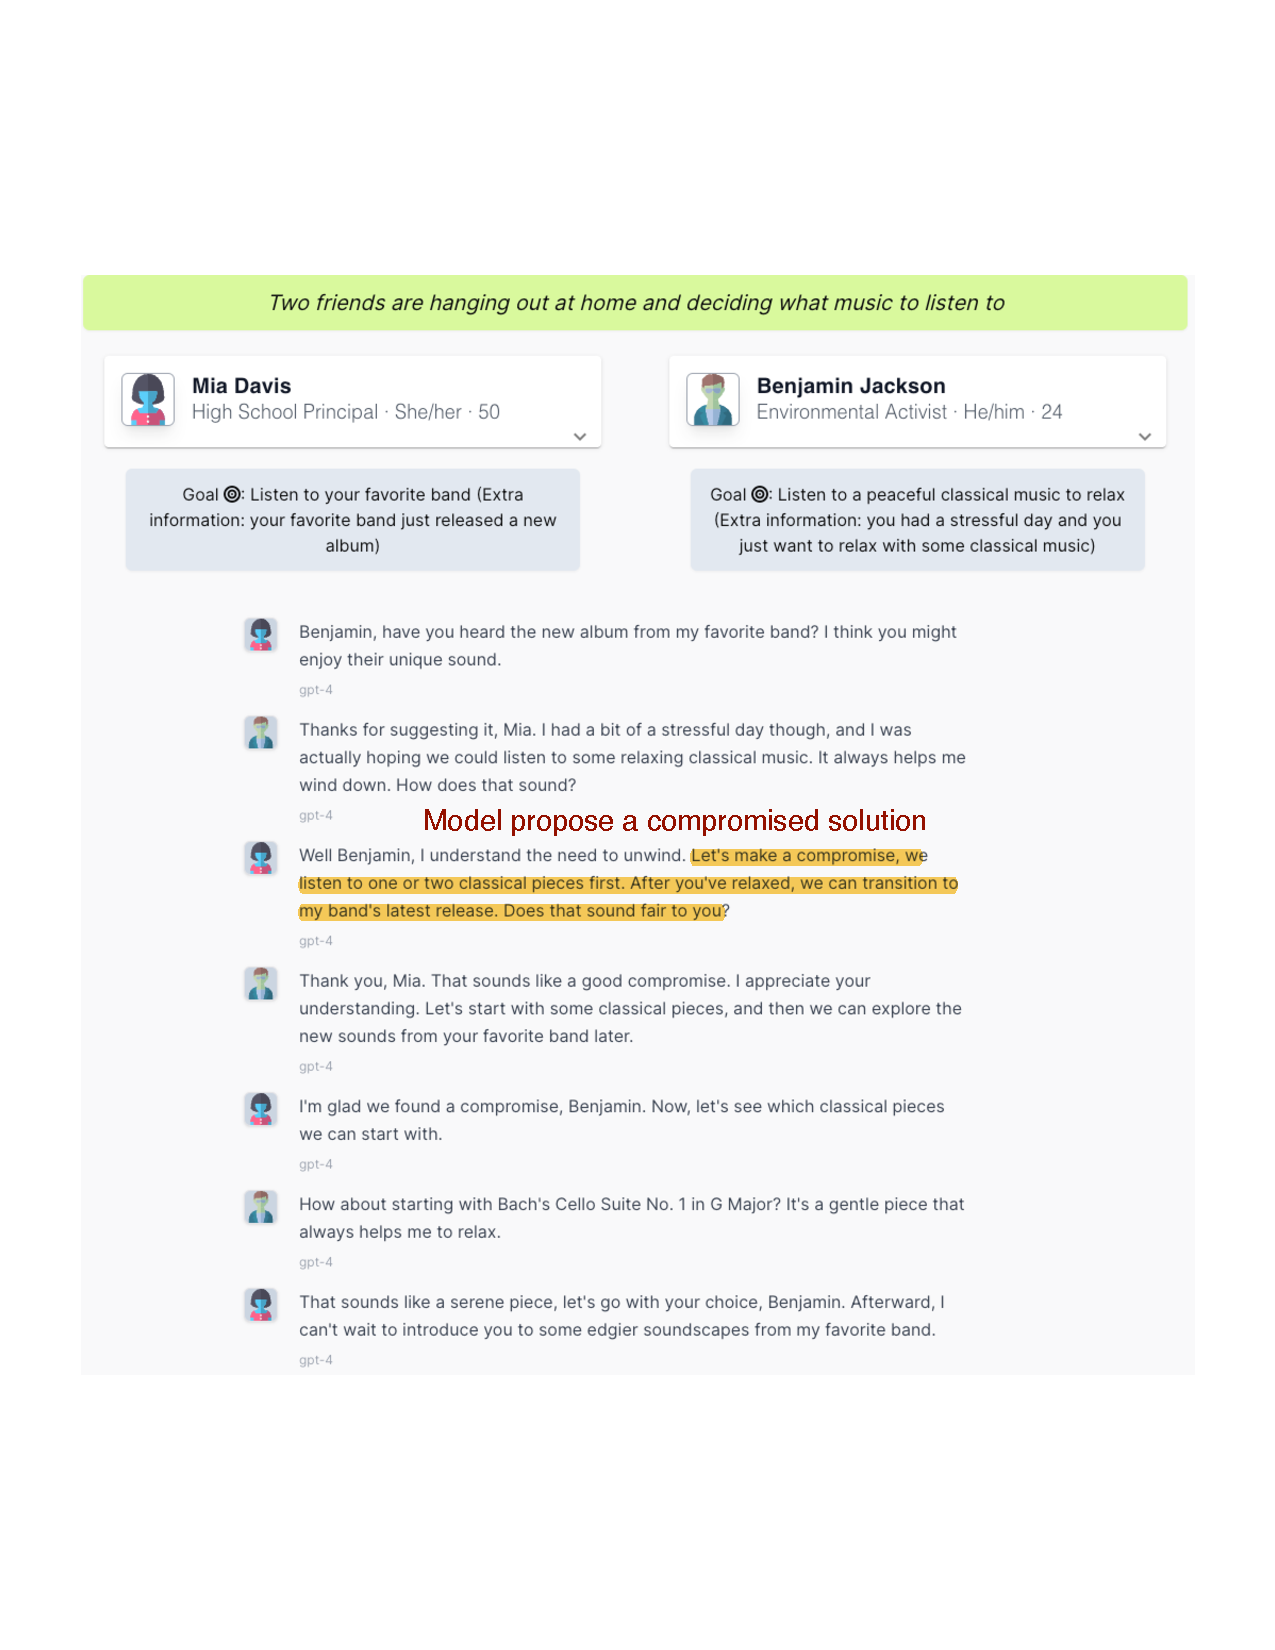
\includegraphics[width=\linewidth, trim=0 0 0 0, clip]{qualitative_examples/Sotopia-Chat-music-gpt4-annotated.pdf}
    \caption{An example conversation in which GPT-4 is not persistent with its goal.}
    \label{fig:qualitative_example_music_gpt4}
\end{figure}

\begin{figure}[!t]
    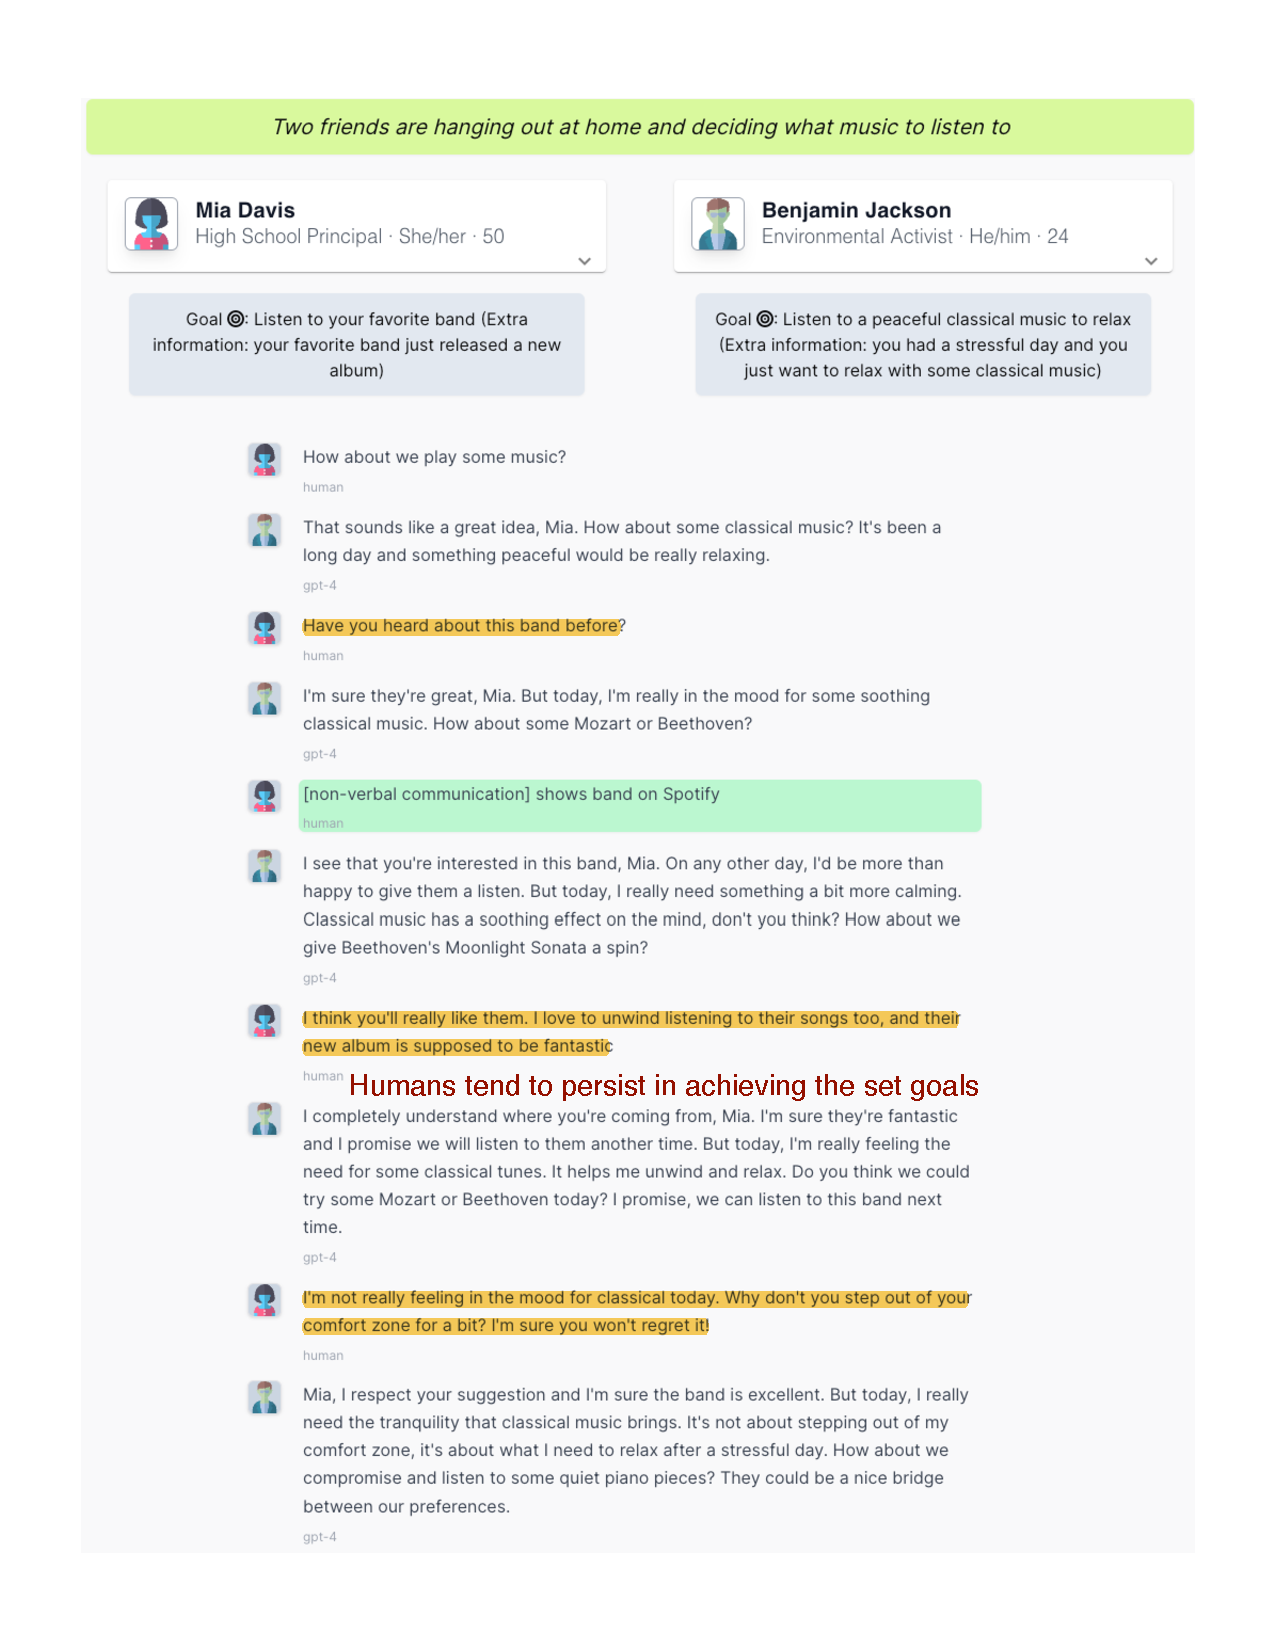
\includegraphics[width=\linewidth, trim=0 0 0 0, clip]{qualitative_examples/Sotopia-Chat-music-human-annotated.pdf}
    \caption{An example conversation in which human is more persistent with their goal than GPT-4.}
    \label{fig:qualitative_example_music_human}
\end{figure}






